\documentclass[dvipdfmx]{jsarticle}
\setcounter{section}{1}
\setcounter{subsection}{3}
\usepackage{xr}
\externaldocument{8.1.1}
\usepackage{amsmath,amsfonts,amssymb,array,comment,mathtools,url,docmute}
\usepackage{longtable,booktabs,dcolumn,tabularx,mathtools,multirow,colortbl,xcolor}
\usepackage[dvipdfmx]{graphics}
\usepackage{bmpsize}
\usepackage{amsthm}
\usepackage{enumitem}
\setlistdepth{20}
\renewlist{itemize}{itemize}{20}
\setlist[itemize]{label=•}
\renewlist{enumerate}{enumerate}{20}
\setlist[enumerate]{label=\arabic*.}
\setcounter{MaxMatrixCols}{20}
\setcounter{tocdepth}{3}
\newcommand{\rotin}{\text{\rotatebox[origin=c]{90}{$\in $}}}
\newcommand{\amap}[6]{\text{\raisebox{-0.7cm}{\begin{tikzpicture} 
  \node (a) at (0, 1) {$\textstyle{#2}$};
  \node (b) at (#6, 1) {$\textstyle{#3}$};
  \node (c) at (0, 0) {$\textstyle{#4}$};
  \node (d) at (#6, 0) {$\textstyle{#5}$};
  \node (x) at (0, 0.5) {$\rotin $};
  \node (x) at (#6, 0.5) {$\rotin $};
  \draw[->] (a) to node[xshift=0pt, yshift=7pt] {$\textstyle{\scriptstyle{#1}}$} (b);
  \draw[|->] (c) to node[xshift=0pt, yshift=7pt] {$\textstyle{\scriptstyle{#1}}$} (d);
\end{tikzpicture}}}}
\newcommand{\twomaps}[9]{\text{\raisebox{-0.7cm}{\begin{tikzpicture} 
  \node (a) at (0, 1) {$\textstyle{#3}$};
  \node (b) at (#9, 1) {$\textstyle{#4}$};
  \node (c) at (#9+#9, 1) {$\textstyle{#5}$};
  \node (d) at (0, 0) {$\textstyle{#6}$};
  \node (e) at (#9, 0) {$\textstyle{#7}$};
  \node (f) at (#9+#9, 0) {$\textstyle{#8}$};
  \node (x) at (0, 0.5) {$\rotin $};
  \node (x) at (#9, 0.5) {$\rotin $};
  \node (x) at (#9+#9, 0.5) {$\rotin $};
  \draw[->] (a) to node[xshift=0pt, yshift=7pt] {$\textstyle{\scriptstyle{#1}}$} (b);
  \draw[|->] (d) to node[xshift=0pt, yshift=7pt] {$\textstyle{\scriptstyle{#2}}$} (e);
  \draw[->] (b) to node[xshift=0pt, yshift=7pt] {$\textstyle{\scriptstyle{#1}}$} (c);
  \draw[|->] (e) to node[xshift=0pt, yshift=7pt] {$\textstyle{\scriptstyle{#2}}$} (f);
\end{tikzpicture}}}}
\renewcommand{\thesection}{第\arabic{section}部}
\renewcommand{\thesubsection}{\arabic{section}.\arabic{subsection}}
\renewcommand{\thesubsubsection}{\arabic{section}.\arabic{subsection}.\arabic{subsubsection}}
\everymath{\displaystyle}
\allowdisplaybreaks[4]
\usepackage{vtable}
\theoremstyle{definition}
\newtheorem{thm}{定理}[subsection]
\newtheorem*{thm*}{定理}
\newtheorem{dfn}{定義}[subsection]
\newtheorem*{dfn*}{定義}
\newtheorem{axs}[dfn]{公理}
\newtheorem*{axs*}{公理}
\renewcommand{\headfont}{\bfseries}
\makeatletter
  \renewcommand{\section}{%
    \@startsection{section}{1}{\z@}%
    {\Cvs}{\Cvs}%
    {\normalfont\huge\headfont\raggedright}}
\makeatother
\makeatletter
  \renewcommand{\subsection}{%
    \@startsection{subsection}{2}{\z@}%
    {0.5\Cvs}{0.5\Cvs}%
    {\normalfont\LARGE\headfont\raggedright}}
\makeatother
\makeatletter
  \renewcommand{\subsubsection}{%
    \@startsection{subsubsection}{3}{\z@}%
    {0.4\Cvs}{0.4\Cvs}%
    {\normalfont\Large\headfont\raggedright}}
\makeatother
\makeatletter
\renewenvironment{proof}[1][\proofname]{\par
  \pushQED{\qed}%
  \normalfont \topsep6\p@\@plus6\p@\relax
  \trivlist
  \item\relax
  {
  #1\@addpunct{.}}\hspace\labelsep\ignorespaces
}{%
  \popQED\endtrivlist\@endpefalse
}
\makeatother
\renewcommand{\proofname}{\textbf{証明}}
\usepackage{tikz,graphics}
\usepackage[dvipdfmx]{hyperref}
\usepackage{pxjahyper}
\hypersetup{
 setpagesize=false,
 bookmarks=true,
 bookmarksdepth=tocdepth,
 bookmarksnumbered=true,
 colorlinks=false,
 pdftitle={},
 pdfsubject={},
 pdfauthor={},
 pdfkeywords={}}
\begin{document}
%\hypertarget{ux8a98ux5c0eux4f4dux76f8ux7a7aux9593}{%
\subsection{誘導位相空間}%\label{ux8a98ux5c0eux4f4dux76f8ux7a7aux9593}}
%\hypertarget{ux8a98ux5c0eux4f4dux76f8ux7a7aux9593-1}{%
\subsubsection{誘導位相空間}%\label{ux8a98ux5c0eux4f4dux76f8ux7a7aux9593-1}}\par
1つの集合$S$と1つの位相空間$\left( T,\mathfrak{P} \right)$、1つの写像$f:S \rightarrow T$が与えられたとき、その写像$f$がある位相空間$\left( S,\mathfrak{O} \right)$からその位相空間$\left( T,\mathfrak{P} \right)$への連続写像となるようなその位相$\mathfrak{O}$を求めたい。しかしながら、このような位相$\mathfrak{O}$が存在したとすれば、これより強い位相$\mathfrak{O}'$を用いて$\forall P \in \mathfrak{P}$に対し、$V\left( f^{- 1}|P \right)\in \mathfrak{O \subseteq}\mathfrak{O}'$が成り立ちその写像$f$はその位相空間$\left( S,\mathfrak{O}' \right)$からその位相空間$\left( T,\mathfrak{P} \right)$への連続写像となるので、その位相$\mathfrak{O}$は必ずしも一意的に決まるとは限らない。
\begin{thm}\label{8.1.4.1}
1つの集合$S$と1つの位相空間$\left( T,\mathfrak{P} \right)$、1つの写像$f:S \rightarrow T$が与えられたとき、その写像$f$がある位相空間$\left( S,\mathfrak{O} \right)$からその位相空間$\left( T,\mathfrak{P} \right)$への連続写像となるような位相たち$\mathfrak{O}$のうち、最も強いものは離散位相$\mathfrak{P}(S)$である。
\end{thm}
\begin{proof}
1つの集合$S$と1つの位相空間$\left( T,\mathfrak{P} \right)$、1つの写像$f:S \rightarrow T$が与えられたとき、その集合$S$を台集合とする離散位相$\mathfrak{P}(S)$について、$\forall P \in \mathfrak{P}$に対し、値域の定義より$V\left( f^{- 1}|P \right)\in \mathfrak{P}(S)$が必ず成り立つ。さらに、その離散位相$\mathfrak{P}(S)$はその集合$S$を台集合とするその写像$f$がある位相空間$\left( S,\mathfrak{O} \right)$からその位相空間$\left( T,\mathfrak{P} \right)$への連続写像となるような任意の位相$\mathfrak{O}$に対し、$\mathfrak{O \subseteq P}(S)$を満たすので、このような位相たち$\mathfrak{O}$のうち、最も強いものはその離散位相$\mathfrak{P}(S)$となる。
\end{proof}
\begin{thm}\label{8.1.4.2}
1つの集合$S$と1つの位相空間$\left( T,\mathfrak{P} \right)$、1つの写像$f:S \rightarrow T$が与えられたとき、その写像$f$がある位相空間$\left( S,\mathfrak{O} \right)$からその位相空間$\left( T,\mathfrak{P} \right)$への連続写像となるような位相たち$\mathfrak{O}$のうち、最も弱いものは次式のように定義されるその位相$\mathfrak{P}$の元$P$のその逆対応$f^{- 1}$による値域$V\left( f^{- 1}|P \right)$全体の集合$\mathfrak{O}_{0}$である。
\begin{align*}
\mathfrak{O}_{0} = \left\{ O'\in \mathfrak{P}(S) \middle| \exists P \in \mathfrak{P}\left[ O' = V\left( f^{- 1}|P \right) \right] \right\}
\end{align*}
\end{thm}
\begin{dfn}
この位相$\mathfrak{O}_{0}$をその写像$f$によってその位相空間$\left( T,\mathfrak{P} \right)$から誘導される位相、その写像$f$によるその位相空間$\left( T,\mathfrak{P} \right)$からの誘導位相、始位相などといいその位相空間$\left( S,\mathfrak{O}_{0} \right)$をその写像$f$によるその位相空間$\left( T,\mathfrak{P} \right)$からの誘導位相空間、始位相空間などという。
\end{dfn}
\begin{proof}
1つの集合$S$と1つの位相空間$\left( T,\mathfrak{P} \right)$、1つの写像$f:S \rightarrow T$が与えられたとし、次式のようにその位相$\mathfrak{P}$の元$P$のその逆対応$f^{- 1}$による値域$V\left( f^{- 1}|P \right)$全体の集合$\mathfrak{O}_{0}$が定義される。
\begin{align*}
\mathfrak{O}_{0} = \left\{ O'\in \mathfrak{P}(S) \middle| \exists P \in \mathfrak{P}\left[ O' = V\left( f^{- 1}|P \right) \right] \right\}
\end{align*}
このとき、位相の定義より$T \in \mathfrak{P}$が成り立つかつ、$D(f) = V\left( f^{- 1} \right)$が成り立つかつ、その対応$f$が写像であるので、$D(f) = S$が成り立つことに注意すれば、$V\left( f^{- 1}|T \right) = S$が成り立つ。さらに、位相の定義より$\mathfrak{\emptyset \in P}$が成り立つので、$V\left( f^{- 1}|\emptyset \right) = \emptyset$が成り立つ。以上より、$S,\emptyset \in \mathfrak{O}_{0}$が成り立つ。任意の添数集合$\varLambda$によって添数づけられたその集合$\mathfrak{O}_{0}$の元の族$\left\{ O_{\lambda} \right\}_{\lambda \in \varLambda}$が与えられたとき、その集合$\mathfrak{O}_{0}$の定義より$\forall\lambda \in \varLambda\exists P_{\lambda}\in \mathfrak{P}$に対し、$O_{\lambda} = V\left( f^{- 1}|P_{\lambda} \right)$が成り立つ。ここで、位相の定義より$\bigcup_{\lambda \in \varLambda} P_{\lambda}\in \mathfrak{P}$が成り立つかつ、次式が成り立つ。
\begin{align*}
V\left( f^{- 1}|\bigcup_{\lambda \in \varLambda} P_{\lambda} \right) &= \bigcup_{\lambda \in \varLambda} {V\left( f^{- 1}|P_{\lambda} \right)}\\
&= \bigcup_{\lambda \in \varLambda} O_{\lambda} \in \mathfrak{O}_{0}
\end{align*}
$\forall O,P \in \mathfrak{O}_{0}$に対し、その集合$\mathfrak{O}_{0}$の定義より$\exists Q,R \in \mathfrak{P}$に対し、$O = V\left( f^{- 1}|Q \right)$かつ$P = V\left( f^{- 1}|R \right)$が成り立つ。ここで、位相の定義より$Q \cap R \in \mathfrak{P}$が成り立つかつ、その対応$f$は写像であり次式が成り立つ。
\begin{align*}
V\left( f^{- 1}|Q \cap R \right) &= V\left( f^{- 1}|Q \right) \cap V\left( f^{- 1}|R \right)\\
&= O \cap P \in \mathfrak{O}_{0}
\end{align*}
以上より、その集合$\mathfrak{O}_{0}$はその集合$S$を台集合とする位相である。また、その位相$\mathfrak{O}_{0}$の定義より$\forall P \in \mathfrak{P}$に対し、$V\left( f^{- 1}|P \right) \in \mathfrak{O}_{0}$が成り立つので、その写像$f$は連続写像である。\par
さらに、その写像$f$がある位相空間$\left( S,\mathfrak{O} \right)$からその位相空間$\left( T,\mathfrak{P} \right)$への連続写像となるとき、$\forall O \in \mathfrak{O}_{0}\exists P \in \mathfrak{P}$に対し、$O = V\left( f^{- 1}|P \right)$が成り立つので、$O = V\left( f^{- 1}|P \right)\in \mathfrak{O}$が成り立つ。したがって、このような位相$\mathfrak{O}$すべて$\mathfrak{O}_{0}\subseteq \mathfrak{O}$を満たす。\par
以上より、このような位相たち$\mathfrak{O}$のうち、最も弱いものはその位相$\mathfrak{O}_{0}$となる。
\end{proof}\par
さらに、1つの集合$S$と添数集合$\varLambda$によって添数づけられた位相空間の族$\left\{ \left( S_{\lambda},\mathfrak{O}_{\lambda} \right) \right\}_{\lambda \in \varLambda}$、その添数集合$\varLambda$によって添数づけられた写像の族$\left\{ f_{\lambda}:S \rightarrow S_{\lambda} \right\}_{\lambda \in \varLambda}$が与えられたとき、$\forall\lambda \in \varLambda$に対し、それらの写像たち$f_{\lambda}$がある位相空間$\left( S,\mathfrak{O} \right)$からその位相空間$\left( S_{\lambda},\mathfrak{O}_{\lambda} \right)$への連続写像となるようなその位相$\mathfrak{O}$を求めたい。
\begin{thm}\label{8.1.4.3}
このような位相$\mathfrak{O}$のうち最も強いものはやはり離散位相$\mathfrak{P}\left( \mathfrak{O} \right)$となる。
\end{thm}
\begin{proof}
1つの集合$S$と添数集合$\varLambda$によって添数づけられた位相空間の族$\left\{ \left( S_{\lambda},\mathfrak{O}_{\lambda} \right) \right\}_{\lambda \in \varLambda}$、その添数集合$\varLambda$によって添数づけられた写像の族$\left\{ f_{\lambda}:S \rightarrow S_{\lambda} \right\}_{\lambda \in \varLambda}$が与えられたとき、その集合$S$を台集合とする離散位相$\mathfrak{P}(S)$について、$\forall\lambda \in \varLambda\forall O_{\lambda} \in \mathfrak{O}_{\lambda}$に対し、値域の定義より$V\left( f^{- 1}|O_{\lambda} \right)\in \mathfrak{P}(S)$が必ず成り立つ。さらに、その離散位相$\mathfrak{P}(S)$はその集合$S$を台集合とする任意の位相たち$\mathfrak{O}$を用いて$\mathfrak{O \subseteq P}(S)$を満たすので、$\forall\lambda \in \varLambda$に対し、それらの写像たち$f_{\lambda}$がある位相空間$\left( S,\mathfrak{O} \right)$からその位相空間$\left( S_{\lambda},\mathfrak{O}_{\lambda} \right)$への連続写像となるような位相たち$\mathfrak{O}$のうち、最も強いものはその離散位相$\mathfrak{P}(S)$となる。
\end{proof}
\begin{thm}\label{8.1.4.4}
このような位相$\mathfrak{O}$のうち最も弱いのは次式のように定義されるその集合$S$を台集合とする位相全体の集合$\mathcal{T}(S)$を用いた順序集合$\left( \mathcal{T}(S), \subseteq \right)$におけるその写像$f_{\lambda}$によるその位相空間$\left( S_{\lambda},\mathfrak{O}_{\lambda} \right)$からの誘導位相$\mathfrak{O}_{\lambda}'$全体の集合の上限$\mathfrak{O}_{0}$である。
\begin{align*}
\mathfrak{O}_{0} = \sup\left\{ \mathfrak{O}_{\lambda}'\in \mathcal{T}(S) \middle| \lambda \in \varLambda \right\}
\end{align*}
\end{thm}
\begin{dfn}
この位相$\mathfrak{O}_{0}$をその写像の族$\left\{ f_{\lambda}:S \rightarrow S_{\lambda} \right\}_{\lambda \in \varLambda}$によってその位相空間の族$\left\{ \left( S_{\lambda},\mathfrak{O}_{\lambda} \right) \right\}_{\lambda \in \varLambda}$から誘導される位相、その写像の族$\left\{ f_{\lambda}:S \rightarrow S_{\lambda} \right\}_{\lambda \in \varLambda}$によるその位相空間の族$\left\{ \left( S_{\lambda},\mathfrak{O}_{\lambda} \right) \right\}_{\lambda \in \varLambda}$からの誘導位相、始位相などといいその位相空間$\left( S,\mathfrak{O}_{0} \right)$をその写像の族$\left\{ f_{\lambda}:S \rightarrow S_{\lambda} \right\}_{\lambda \in \varLambda}$によるその位相空間の族$\left\{ \left( S_{\lambda},\mathfrak{O}_{\lambda} \right) \right\}_{\lambda \in \varLambda}$からの誘導位相空間、始位相空間などという。
\end{dfn}
\begin{proof}
1つの集合$S$と添数集合$\varLambda$によって添数づけられた位相空間の族$\left\{ \left( S_{\lambda},\mathfrak{O}_{\lambda} \right) \right\}_{\lambda \in \varLambda}$、その添数集合$\varLambda$によって添数づけられた写像の族$\left\{ f_{\lambda}:S \rightarrow S_{\lambda} \right\}_{\lambda \in \varLambda}$が与えられたとき、$\forall\lambda \in \varLambda$に対し、その写像$f_{\lambda}$によるその位相空間$\left( S_{\lambda},\mathfrak{O}_{\lambda} \right)$からの誘導位相を$\mathfrak{O}_{\lambda}'$とおくと、それらの写像たち$f_{\lambda}$がその位相空間$\left( S,\mathfrak{O}_{\lambda}' \right)$からその位相空間$\left( S_{\lambda},\mathfrak{O}_{\lambda} \right)$への連続写像となり、$\forall\lambda \in \varLambda\forall O_{\lambda} \in \mathfrak{O}_{\lambda}$に対し、$V\left( f^{- 1}|O_{\lambda} \right) \in \mathfrak{O}_{\lambda}'$が成り立つ。その集合$S$を台集合とする位相全体の集合$\mathcal{T}$を用いた順序集合$\left( \mathcal{T}(S), \subseteq \right)$を考え、それらの誘導位相$\mathfrak{O}_{\lambda}'$全体の集合$\left\{ \mathfrak{O}_{\lambda}'\in \mathcal{T}(S) \middle| \lambda \in \varLambda \right\}$の任意の上界$\mathfrak{O}'$、即ち、$\forall\lambda \in \varLambda$に対し、$\mathfrak{O}_{\lambda}' \subseteq \mathfrak{O}'$が成り立つような任意の位相$\mathfrak{O}'$は、$\forall\lambda \in \varLambda\forall O_{\lambda} \in \mathfrak{O}_{\lambda}$に対し、$V\left( f^{- 1}|O_{\lambda} \right) \in \mathfrak{O}'$を満たすので、その位相$\mathfrak{O}'$は、$\forall\lambda \in \varLambda$に対し、それらの写像たち$f_{\lambda}$がある位相空間$\left( S,\mathfrak{O} \right)$からその位相空間$\left( S_{\lambda},\mathfrak{O}_{\lambda} \right)$への連続写像となる。ここで、それらの誘導位相$\mathfrak{O}_{\lambda}'$全体の集合$\left\{ \mathfrak{O}_{\lambda}'\in \mathcal{T}(S) \middle| \lambda \in \varLambda \right\}$はその集合$\mathcal{T}(S)$の元の族でありこの集合$\left\{ \mathfrak{O}_{\lambda}'\in \mathcal{T}(S) \middle| \lambda \in \varLambda \right\}$の上限がその集合$\mathcal{T}(S)$に存在するのであったので、$\forall\lambda \in \varLambda$に対し、それらの写像たち$f_{\lambda}$がある位相空間$\left( S,\mathfrak{O} \right)$からその位相空間$\left( S_{\lambda},\mathfrak{O}_{\lambda} \right)$への連続写像となるような位相$\mathfrak{O}'$全体の集合のうち最も弱いものがその順序集合$\left( \mathcal{T, \subseteq} \right)$における上限$\sup\left\{ \mathfrak{O}_{\lambda}'\in \mathcal{T}(S) \middle| \lambda \in \varLambda \right\}$となる。
\end{proof}
\begin{thm}\label{8.1.4.5}
写像の族$\left\{ f_{\lambda}:S \rightarrow S_{\lambda} \right\}_{\lambda \in \varLambda}$によるその位相空間の族$\left\{ \left( S_{\lambda},\mathfrak{O}_{\lambda} \right) \right\}_{\lambda \in \varLambda}$からの誘導位相$\mathfrak{O}_{0}$は次式を満たす、即ち、その和集合$\bigcup_{\lambda \in \varLambda} \mathfrak{O}_{\lambda}$で生成される位相$\mathfrak{O}\left( \bigcup_{\lambda \in \varLambda} \mathfrak{O}_{\lambda}' \right)$に等しい。
\begin{align*}
\mathfrak{O}_{0} = \mathfrak{O}\left( \bigcup_{\lambda \in \varLambda} \mathfrak{O}_{\lambda}' \right)
\end{align*}
さらに、集合$\mathfrak{B}$が次式のように定義されると、
\begin{align*}
\mathfrak{B} = \left\{ \bigcap_{\scriptsize \begin{matrix}
\mu \in M \\
\end{matrix}} A_{\mu}\in \mathfrak{P}(S) \middle| {\#}M < \aleph_{0},\ \ \forall\mu \in M\left[ A_{\mu} \in \bigcup_{\lambda \in \varLambda} \mathfrak{O}_{\lambda}' \right] \right\}
\end{align*}
次式が成り立つ、
\begin{align*}
\mathfrak{O}_{0} = \left\{ \bigcup_{\nu \in N} B_{\nu}\in \mathfrak{P}(S) \middle| \forall\nu \in N\left[ B_{\nu}\in \mathfrak{B} \right] \right\}
\end{align*}
即ち、その誘導位相$\mathfrak{O}_{0}$はその和集合$\bigcup_{\lambda \in \varLambda} \mathfrak{O}_{\lambda}$を用いて$A_{\mu} \in \bigcup_{\lambda \in \varLambda} \mathfrak{O}_{\lambda}$なる有限個の集合たち$A_{\mu}$の共通部分$\bigcap_{\scriptsize \begin{matrix}
\mu \in M \\
\end{matrix}} A_{\mu}$全体の集合$\mathfrak{B}$を用いて$B_{\nu} \in \mathfrak{B}$なる集合$B_{\nu}$の和集合$\bigcup_{\nu \in N} B_{\nu}$で表される集合全体の集合である。
\end{thm}
\begin{proof}
1つの集合$S$と添数集合$\varLambda$によって添数づけられた位相空間の族$\left\{ \left( S_{\lambda},\mathfrak{O}_{\lambda} \right) \right\}_{\lambda \in \varLambda}$、その添数集合$\varLambda$によって添数づけられた写像の族$\left\{ f_{\lambda}:S \rightarrow S_{\lambda} \right\}_{\lambda \in \varLambda}$が与えられたとき、写像の族$\left\{ f_{\lambda}:S \rightarrow S_{\lambda} \right\}_{\lambda \in \varLambda}$によるその位相空間の族$\left\{ \left( S_{\lambda},\mathfrak{O}_{\lambda} \right) \right\}_{\lambda \in \varLambda}$からの誘導位相$\mathfrak{O}_{0}$は次式のようにその集合$S$を台集合とする位相全体の集合$\mathcal{T}(S)$を用いた順序集合$\left( \mathcal{T}(S), \subseteq \right)$におけるその写像$f_{\lambda}$によるその位相空間$\left( S_{\lambda},\mathfrak{O}_{\lambda} \right)$からの誘導位相$\mathfrak{O}_{\lambda}'$全体の集合の上限$\mathfrak{O}_{0}$であるのであった。
\begin{align*}
\mathfrak{O}_{0} = \sup\left\{ \mathfrak{O}_{\lambda}'\in \mathcal{T}(S) \middle| \lambda \in \varLambda \right\}
\end{align*}
ここで、$\forall\lambda \in \varLambda$に対し、$\mathfrak{O}_{\lambda}' \subseteq \bigcup_{\lambda \in \varLambda} \mathfrak{O}_{\lambda}'$が成り立ち、$\forall\lambda \in \varLambda$に対し、$\mathfrak{O}_{\lambda}' \subseteq \mathfrak{O}'$が成り立つならそのときに限り、$\bigcup_{\lambda \in \varLambda} \mathfrak{O}_{\lambda}' \subseteq \mathfrak{O}'$が成り立つので、集合$\mathfrak{O}'$がその集合$\left\{ \mathfrak{O}_{\lambda}'\in \mathcal{T}(S) \middle| \lambda \in \varLambda \right\}$の上界であるならそのときに限り、$\bigcup_{\lambda \in \varLambda} \mathfrak{O}_{\lambda}' \subseteq \mathfrak{O}'$が成り立つことになる。したがって、その集合$\left\{ \mathfrak{O}_{\lambda}'\in \mathcal{T}(S) \middle| \lambda \in \varLambda \right\}$の上限$\sup\left\{ \mathfrak{O}_{\lambda}'\in \mathcal{T} \middle| \lambda \in \varLambda \right\}$は$\bigcup_{\lambda \in \varLambda} \mathfrak{O}_{\lambda}' \subseteq \mathfrak{O}'$が成り立つような位相$\mathfrak{O}'$のうち最も弱いので、定義より$\mathfrak{O}_{0} = \mathfrak{O}\left( \bigcup_{\lambda \in \varLambda} \mathfrak{O}_{\lambda}' \right)$のようにその位相$\mathfrak{O}_{0}$はその集合$\bigcup_{\lambda \in \varLambda} \mathfrak{O}_{\lambda}'$で生成される位相$\mathfrak{O}\left( \bigcup_{\lambda \in \varLambda} \mathfrak{O}_{\lambda}' \right)$である。\par
このとき、その位相$\mathfrak{O}_{0}$は、有限集合である添数集合$M$によって添数づけられたその集合$\bigcup_{\lambda \in \varLambda} \mathfrak{O}_{\lambda}'$の元の族$\left\{ A_{\mu} \right\}_{\mu \in M}$の積集合全体の集合を$\mathfrak{B}$として、任意の添数集合$N$によって添数づけられたその集合$\mathfrak{B}$の元の族$\left\{ B_{\nu} \right\}_{\nu \in N}$の和集合全体の集合に等しいのであったので、集合$\mathfrak{B}$が次式のように定義されると、
\begin{align*}
\mathfrak{B} =\left\{ \bigcap_{\scriptsize \begin{matrix}
\mu \in M \\
\end{matrix}} A_{\mu}\in \mathfrak{P}(S) \middle| {\#}M < \aleph_{0},\ \ \forall\mu \in M\left[ A_{\mu} \in \bigcup_{\lambda \in \varLambda} \mathfrak{O}_{\lambda}' \right] \right\}
\end{align*}
次式が成り立つ。
\begin{align*}
\mathfrak{O}_{0} = \left\{ \bigcup_{\nu \in N} B_{\nu}\in \mathfrak{P}(S) \middle| \forall\nu \in N\left[ B_{\nu}\in \mathfrak{B} \right] \right\}
\end{align*}
\end{proof}
\begin{thm}\label{8.1.4.6}
写像の族$\left\{ f_{\lambda}:S \rightarrow S_{\lambda} \right\}_{\lambda \in \varLambda}$によるその位相空間の族$\left\{ \left( S_{\lambda},\mathfrak{O}_{\lambda} \right) \right\}_{\lambda \in \varLambda}$からの誘導位相$\mathfrak{O}_{0}$において、その写像$f_{\lambda}$によるその位相空間$\left( S_{\lambda},\mathfrak{O}_{\lambda} \right)$からの誘導位相$\mathfrak{O}_{\lambda}'$を用いて集合$\mathfrak{B}$が次式のように定義されると、
\begin{align*}
\mathfrak{B} = \left\{ \bigcap_{\scriptsize \begin{matrix}
\mu \in M \\
\end{matrix}} A_{\mu}\in \mathfrak{P}(S) \middle| {\#}M < \aleph_{0},\ \ \forall\mu \in M\left[ A_{\mu} \in \bigcup_{\lambda \in \varLambda} \mathfrak{O}_{\lambda}' \right] \right\}
\end{align*}
その集合$\mathfrak{B}$はその位相空間$\left( S,\mathfrak{O}_{0} \right)$の1つの開基となる。さらに、$\forall W \in \mathfrak{B}$に対し、その添数集合$\varLambda$の有限集合である添数集合$N$の添数$\nu$につき$O_{\nu} \in \mathfrak{O}_{\nu}$なる開集合たち$O_{\nu}$を用いて次式のように書かれることができる。
\begin{align*}
W = \bigcap_{\scriptsize \begin{matrix}
\nu \in N \\
\end{matrix}} {V\left( f_{\nu}^{- 1}|O_{\nu} \right)}
\end{align*}
\end{thm}
\begin{proof}
写像の族$\left\{ f_{\lambda}:S \rightarrow S_{\lambda} \right\}_{\lambda \in \varLambda}$によるその位相空間の族$\left\{ \left( S_{\lambda},\mathfrak{O}_{\lambda} \right) \right\}_{\lambda \in \varLambda}$からの誘導位相$\mathfrak{O}_{0}$において、その写像$f_{\lambda}$によるその位相空間$\left( S_{\lambda},\mathfrak{O}_{\lambda} \right)$からの誘導位相$\mathfrak{O}_{\lambda}'$を用いて集合$\mathfrak{B}$が次式のように定義されると、
\begin{align*}
\mathfrak{B} =\left\{ \bigcap_{\scriptsize \begin{matrix}
\mu \in M \\
\end{matrix}} A_{\mu}\in \mathfrak{P}(S) \middle| {\#}M < \aleph_{0},\ \ \forall\mu \in M\left[ A_{\mu} \in \bigcup_{\lambda \in \varLambda} \mathfrak{O}_{\lambda}' \right] \right\}
\end{align*}
次式が成り立つので、
\begin{align*}
\mathfrak{O}_{0} = \left\{ \bigcup_{\nu \in N} B_{\nu}\in \mathfrak{P}(S) \middle| \forall\nu \in N\left[ B_{\nu}\in \mathfrak{B} \right] \right\}
\end{align*}
その位相$\mathfrak{O}_{0}$に属する任意の開集合$O$は添数集合$N$によって添数づけられたその集合$\mathfrak{B}$の元の族$\left\{ B_{\nu} \right\}_{\nu \in N}$の和集合$\bigcup_{\nu \in N} B_{\nu}$であるので、定義よりその集合$\mathfrak{B}$はその位相空間$\left( S,\mathfrak{O}_{0} \right)$の1つの開基である。\par
さらに、その開基$\mathfrak{B}$の任意の元$W$は、有限集合である添数集合$M$の添数$\mu$に対し、$O_{\mu} \in \bigcup_{\lambda \in \varLambda} \mathfrak{O}_{\lambda}'$なる開集合たち$O_{\mu}$を用いて$W = \bigcap_{\scriptsize \begin{matrix}
\mu \in M \\
\end{matrix}} O_{\mu}$を満たす。ここで、${\#}M = 1$のとき、$\mu \in M$なる添数$\mu$を用いて$O_{\mu} \in \bigcup_{\lambda \in \varLambda} \mathfrak{O}_{\lambda}'$が成り立つので、$O_{\mu} \in \mathfrak{O}_{\lambda}'$が成り立つような添数$\lambda$がその添数集合$\varLambda$に存在する。次式が成り立つのであったので、
\begin{align*}
\mathfrak{O}_{\lambda}' = \left\{ O'\in \mathfrak{P}(S) \middle| \exists O_{\lambda} \in \mathfrak{O}_{\lambda}\left[ O' = V\left( f_{\lambda}^{- 1}|O_{\lambda} \right) \right] \right\}
\end{align*}
その位相$\mathfrak{O}_{\lambda}'$のある開集合$O_{\lambda}$を用いて$O_{\mu} = V\left( f_{\lambda}^{- 1}|O_{\lambda} \right)$が成り立つ。\par
${\#}M = k$のときに示すべきことが成り立つと仮定しよう。${\#}M = k + 1$のとき、その添数集合$M$の1つの添数$\mu'$を用いれば、仮定よりその添数集合$\varLambda$の有限集合であるある部分集合$\varLambda'$が存在して、次のようになる。
\begin{align*}
\bigcap_{\scriptsize \begin{matrix}
\mu \in M \\
\end{matrix}} O_{\mu} &= \bigcap_{\scriptsize \begin{matrix}
\mu \in M \setminus \left\{ \mu' \right\} \\
\end{matrix}} O_{\mu} \cap O_{\mu'}\\
&= \bigcap_{\scriptsize \begin{matrix}
\lambda \in \varLambda' \\
\end{matrix}} {V\left( f_{\lambda}^{- 1}|O_{\lambda} \right)} \cap O_{\mu'}
\end{align*}
$O_{\mu'} \in \bigcup_{\lambda \in \varLambda} \mathfrak{O}_{\lambda}'$が成り立つので、$O_{\mu'} \in \mathfrak{O}_{\lambda'}'$が成り立つような添数$\lambda'$がその添数集合$\varLambda$に存在する。次式が成り立つのであったので、
\begin{align*}
\mathfrak{O}_{\lambda'}' = \left\{ O'\in \mathfrak{P}(S) \middle| \exists O_{\lambda'} \in \mathfrak{O}_{\lambda'}\left[ O' = V\left( f_{\lambda'}^{- 1}|O_{\lambda'} \right) \right] \right\}
\end{align*}
$\exists O_{\lambda'} \in \mathfrak{O}_{\lambda'}'$に対し、$O_{\mu'} = V\left( f_{\lambda'}^{- 1}|O_{\lambda'} \right)$が成り立つ。ここで、${\#}\left( \varLambda' \cup \left\{ \lambda' \right\} \right) < \aleph_{0}$が成り立つことに注意すれば、次のようになる。
\begin{align*}
\bigcap_{\scriptsize \begin{matrix}
\mu \in M \\
\end{matrix}} O_{\mu} &= \bigcap_{\scriptsize \begin{matrix}
\lambda \in \varLambda' \\
\end{matrix}} {V\left( f_{\lambda}^{- 1}|O_{\lambda} \right)} \cap V\left( f_{\lambda'}^{- 1}|O_{\lambda'} \right)\\
&= \bigcap_{\scriptsize \begin{matrix}
\lambda \in \varLambda' \cup \left\{ \lambda' \right\} \\
\end{matrix}} {V\left( f_{\lambda}^{- 1}|O_{\lambda} \right)}
\end{align*}\par
以上より数学的帰納法によって、その添数集合$\varLambda$の有限集合であるある部分集合$\varLambda'$の添数$\lambda$に対し、$O_{\lambda} \in \mathfrak{O}_{\lambda}$なる開集合たち$O_{\lambda}$を用いて次式が成り立つ。
\begin{align*}
W &= \bigcap_{\scriptsize \begin{matrix}
\mu \in M \\
\end{matrix}} O_{\mu}\\
&= \bigcap_{\scriptsize \begin{matrix}
\lambda \in \varLambda' \\
\end{matrix}} {V\left( f_{\lambda}^{- 1}|O_{\lambda} \right)}
\end{align*}
\end{proof}
%\hypertarget{ux76f8ux5bfeux4f4dux76f8ux7a7aux9593}{%
\subsubsection{相対位相空間}%\label{ux76f8ux5bfeux4f4dux76f8ux7a7aux9593}}
\begin{dfn}
1つの位相空間$\left( S,\mathfrak{O} \right)$において、その集合$S$の空でない部分集合$M$からその集合$S$への包含写像$M \hookrightarrow S;a \mapsto a$が与えられたとする。このとき、その集合$M$を台集合とするその写像$M \hookrightarrow S$によるその位相空間$\left( S,\mathfrak{O} \right)$からの誘導位相$\mathfrak{O}_{M}$をその集合$M$におけるその位相空間$\left( S,\mathfrak{O} \right)$の相対位相といいその位相空間$\left( M,\mathfrak{O}_{M} \right)$をその集合$M$におけるその位相空間$\left( S,\mathfrak{O} \right)$の部分位相空間、部分空間などという。
\end{dfn}\par
定義より明らかに、その写像$M \hookrightarrow S$がその部分位相空間$\left( M,\mathfrak{O}' \right)$からその位相空間$\left( S,\mathfrak{O} \right)$への連続写像となるような位相たち$\mathfrak{O}'$のうち、その相対位相$\mathfrak{O}_{M}$が最も弱い。
\begin{thm}\label{8.1.4.7}
位相空間$\left( S,\mathfrak{O} \right)$の台集合$S$の空でない部分集合$M$が与えられたとする。集合$M$における位相空間$\left( S,\mathfrak{O} \right)$の相対位相$\mathfrak{O}_{M}$について、その位相空間$\left( S,\mathfrak{O} \right)$の閉集合系を$\mathfrak{A}$、$a \in M$なる元$a$における全近傍系を$\mathbf{V}(a)$、その部分位相空間$\left( M,\mathfrak{O}_{M} \right)$の閉集合系を$\mathfrak{A}_{M}$、その元$a$における全近傍系を$\mathbf{V}_{M}(a)$とおくと、$\forall a \in M$に対し、次式が成り立つ。
\begin{align*}
\mathfrak{O}_{M} &= \left\{ O'\in \mathfrak{P}(M) \middle| \exists O \in \mathfrak{O}\left[ O' = O \cap M \right] \right\}\\
\mathfrak{A}_{M} &= \left\{ A'\in \mathfrak{P}(M) \middle| \exists A \in \mathfrak{A}\left[ A' = A \cap M \right] \right\}\\
\mathbf{V}_{M}(a) &= \left\{ V'\in \mathfrak{P}(M) \middle| \exists V \in \mathbf{V}(a)\left[ V' = V \cap M \right] \right\}
\end{align*}
\end{thm}
\begin{proof}
1つの位相空間$\left( S,\mathfrak{O} \right)$において、その集合$S$の空でない部分集合$M$が与えられたとする。集合$M$における位相空間$\left( S,\mathfrak{O} \right)$の相対位相$\mathfrak{O}_{M}$について、その位相空間$\left( S,\mathfrak{O} \right)$の閉集合系を$\mathfrak{A}$、$a \in M$なる元$a$における全近傍系を$\mathbf{V}(a)$、その部分位相空間$\left( M,\mathfrak{O}_{M} \right)$の閉集合系を$\mathfrak{A}_{M}$、その元$a$における全近傍系を$\mathbf{V}_{M}(a)$とおくと、その集合$M$における位相空間$\left( S,\mathfrak{O} \right)$の相対位相$\mathfrak{O}_{M}$は定義より明らかに包含写像$M \hookrightarrow S$によるその位相空間$\left( S,\mathfrak{O} \right)$からの誘導位相であり、これについて、次式が成り立つのであった。
\begin{align*}
\mathfrak{O}_{M} = \left\{ O'\in \mathfrak{P}(M) \middle| \exists O \in \mathfrak{O}\left[ O' = V\left( (M \hookrightarrow S)^{- 1}|O \right) \right] \right\}
\end{align*}
ここで、$\forall a \in V\left( (M \hookrightarrow S)^{- 1}|O \right)$に対し、値域の定義より$(M \hookrightarrow S)(a) = b$となるような元$b$がその集合$O$に存在し、その写像$M \hookrightarrow S$の定義より、$a = b$が成り立つので、$a \in O \cap M$が成り立ち$V\left( (M \hookrightarrow S)^{- 1}|O \right) = O \cap M$が成り立つ。これにより、次式が成り立つ。
\begin{align*}
\mathfrak{O}_{M} = \left\{ O'\in \mathfrak{P}(M) \middle| \exists O \in \mathfrak{O}\left[ O' = O \cap M \right] \right\}
\end{align*}\par
$\forall A' \in \mathfrak{A}_{M}$に対し、$\exists O' \in \mathfrak{O}_{M}$に対し、$A' = M \setminus O'$が成り立ち、したがって、$O' = M \setminus A'$が成り立つ。ここで、$\mathfrak{O}_{M} = \left\{ O'\in \mathfrak{P}(M) \middle| \exists O \in \mathfrak{O}\left[ O' = O \cap M \right] \right\}$が成り立つので、$\exists A \in \mathfrak{A}$に対し、$M \setminus A' = O' = (S \setminus A) \cap M$が成り立つ。したがって、次のようになり、
\begin{align*}
A' &= M \setminus \left( M \setminus A' \right)\\
&= M \setminus \left( (S \setminus A) \cap M \right)\\
&= M \setminus (S \setminus A) \cup M \setminus M\\
&= M \setminus (S \setminus A)\\
&= M \setminus S \cup (M \cap A)\\
&= A \cap M
\end{align*}
以上の議論が必要十分条件であることに注意すれば、よって、次式が成り立つ。
\begin{align*}
\mathfrak{A}_{M} = \left\{ A'\in \mathfrak{P}(M) \middle| \exists A \in \mathfrak{A}\left[ A' = A \cap M \right] \right\}
\end{align*}\par
また、$\forall a \in M\forall V' \in \mathbf{V}_{M}(a)$に対し、$a \in {\mathrm{int}}V'$が成り立つかつ、$V' \subseteq M$が成り立つ。ここで、$V' \subseteq M$が成り立つならそのときに限り、$V' \cap M = V'$が成り立つので、$a \in {\mathrm{int}}\left( V' \cap M \right)$が成り立つ。さらに、$V' \subseteq S$も成り立つので、$V' \in \mathbf{V}(a)$も成り立つことに注意すれば、$\exists V \in \mathbf{V}(a)$に対し、$V' = V \cap M$が成り立ち、以上の議論が必要十分条件であることに注意すれば、よって、次式が成り立つ。
\begin{align*}
\mathbf{V}_{M}(a) = \left\{ V'\in \mathfrak{P}(M) \middle| \exists V \in \mathbf{V}(a)\left[ V' = V \cap M \right] \right\}
\end{align*}
\end{proof}
\begin{thm}\label{8.1.4.8}
位相空間$\left( S,\mathfrak{O} \right)$の台集合$S$の空でない部分集合$M$が与えられたとする。集合$M$における位相空間$\left( S,\mathfrak{O} \right)$の相対位相$\mathfrak{O}_{M}$について、その位相空間$\left( S,\mathfrak{O} \right)$の閉集合系を$\mathfrak{A}$、$a \in M$なる元$a$における全近傍系を$\mathbf{V}(a)$、その部分位相空間$\left( M,\mathfrak{O}_{M} \right)$の閉集合系を$\mathfrak{A}_{M}$、その元$a$における全近傍系を$\mathbf{V}_{M}(a)$とおくと、次のことが成り立つ。
\begin{itemize}
\item
  $\forall O'\in \mathfrak{P}(M)$に対し、$O' \in \mathfrak{O}_{M}$が成り立つならそのときに限り、$\exists O \in \mathfrak{O}$に対し、$O' = O \cap M$が成り立つ。
\item
  $\forall A'\in \mathfrak{P}(M)$に対し、$A' \in \mathfrak{A}_{M}$が成り立つならそのときに限り、$\exists A \in \mathfrak{A}$に対し、$A' = A \cap M$が成り立つ。
\item
  $\forall a \in M\forall V' \in \mathbf{V}(a)$に対し、$V' \in \mathbf{V}_{M}(a)$が成り立つならそのときに限り、$\exists V \in \mathbf{V}(a)$に対し、$V' = V \cap M$が成り立つ。
\end{itemize}
\end{thm}
\begin{proof} 定理\ref{8.1.4.7}より明らかである。
\end{proof}
\begin{thm}\label{8.1.4.9}
位相空間$\left( S,\mathfrak{O} \right)$の台集合$S$の空でない部分集合$M$が与えられ、その位相空間$\left( S,\mathfrak{O} \right)$の閉包作用子、その部分位相空間$\left( M,\mathfrak{O}_{M} \right)$の閉包作用子をそれぞれ$cl$、${\mathrm{cl}}_{M}$とおくと、$\forall M'\in \mathfrak{P}(M)$に対し、${\mathrm{cl}}_{M}M' = {\mathrm{cl}}M' \cap M$が成り立つ。
\end{thm}
\begin{proof}
1つの位相空間$\left( S,\mathfrak{O} \right)$において、その集合$S$の空でない部分集合$M$が与えられ、その位相空間$\left( S,\mathfrak{O} \right)$の閉包作用子、その部分位相空間$\left( M,\mathfrak{O}_{M} \right)$の閉包作用子をそれぞれ$cl$、${\mathrm{cl}}_{M}$、その位相空間$\left( S,\mathfrak{O} \right)$の閉集合系、その部分位相空間$\left( M,\mathfrak{O}_{M} \right)$の閉集合系をそれぞれ$\mathfrak{A}$、$\mathfrak{A}_{M}$とおくと、$\forall M'\in \mathfrak{P}(M)$に対し、$\forall A' \in \mathfrak{A}_{M}$に対し、次式が成り立つので、
\begin{align*}
\mathfrak{A}_{M} = \left\{ A'\in \mathfrak{P}(M) \middle| \exists A \in \mathfrak{A}\left[ A' = A \cap M \right] \right\}
\end{align*}
$\exists A \in \mathfrak{A}$に対し、$M' \subseteq A' = A \cap M \subseteq A$が成り立ち、したがって、${\mathrm{cl}}M \subseteq {\mathrm{cl}}A = A$が成り立つ。\par
逆に、$\exists A \in \mathfrak{A}$に対し、$A' = A \cap M$が成り立って、${\mathrm{cl}}M' \subseteq A$が成り立つなら、$M' \subseteq {\mathrm{cl}}M' \subseteq A$が成り立つかつ、$M' \subseteq M$が成り立つので、次のようになる。
\begin{align*}
M' &= M' \cap M\\
&\subseteq A \cap M = A'
\end{align*}
これにより、$\forall A' \in \mathfrak{A}_{M}$に対し、$M' \subseteq A'$が成り立つならそのときに限り、$\exists A \in \mathfrak{A}$に対し、$A' = A \cap M$かつ${\mathrm{cl}}M' \subseteq A$が成り立つ。$M' \subseteq {\mathrm{cl}}M'$かつ$M' \subseteq M$が成り立つので、次のようになる。
\begin{align*}
M' &= M' \cap M\\
&\subseteq {\mathrm{cl}}M' \cap M\\
&\subseteq A \cap M = A'
\end{align*}
定義よりしたがって、${\mathrm{cl}}_{M}M' = {\mathrm{cl}}M' \cap M$が成り立つ。
\end{proof}
\begin{thm}\label{8.1.4.10}
位相空間$\left( S,\mathfrak{O} \right)$の台集合$S$の空でない部分集合$M$におけるその位相空間$\left( S,\mathfrak{O} \right)$の部分位相空間$\left( M,\mathfrak{O}_{M} \right)$が与えられたとする。このとき、次のことが成り立つ。
\begin{itemize}
\item
  集合$\mathfrak{M}$がその位相空間$\left( S,\mathfrak{O} \right)$の準開基であるとき、次式のような集合$\mathfrak{M}_{M}$はその部分位相空間$\left( M,\mathfrak{O}_{M} \right)$の準開基となる。
\begin{align*}
\mathfrak{M}_{M} = \left\{ O'\in \mathfrak{P}(M) \middle| \exists O \in \mathfrak{M}\left[ O' = O \cap M \right] \right\}
\end{align*}
\item
  集合$\mathfrak{B}$がその位相空間$\left( S,\mathfrak{O} \right)$の開基であるとき、次式のような集合$\mathfrak{B}_{M}$はその部分位相空間$\left( M,\mathfrak{O}_{M} \right)$の開基となる。
\begin{align*}
\mathfrak{B}_{M} = \left\{ W'\in \mathfrak{P}(M) \middle| \exists W \in \mathfrak{B}\left[ W' = W \cap M \right] \right\}
\end{align*}
\end{itemize}
\end{thm}
\begin{proof}
1つの位相空間$\left( S,\mathfrak{O} \right)$において、その集合$S$の空でない部分集合$M$におけるその位相空間$\left( S,\mathfrak{O} \right)$の部分位相空間$\left( M,\mathfrak{O}_{M} \right)$が与えられたとする。\par
集合$\mathfrak{M}$がその位相空間$\left( S,\mathfrak{O} \right)$の準開基であるとき、定義よりその集合$\mathfrak{M}$で生成される位相$\mathfrak{O}\left( \mathfrak{M} \right)$がその位相$\mathfrak{O}$に等しい。ここで、次式のように集合$\mathfrak{M}_{M}$が定義されると、
\begin{align*}
\mathfrak{M}_{M} = \left\{ O'\in \mathfrak{P}(M) \middle| \exists O \in \mathfrak{M}\left[ O' = O \cap M \right] \right\}
\end{align*}
その集合$\mathfrak{M}_{M}$で生成される位相$\mathfrak{O}\left( \mathfrak{M}_{M} \right)$は、有限集合である添数集合$\varLambda$によって添数づけられたその集合$\mathfrak{M}_{M}$の元の族$\left\{ A_{\lambda} \right\}_{\scriptsize \begin{matrix}
\lambda \in \varLambda \\
\end{matrix}}$の積集合$\bigcap_{\scriptsize \begin{matrix}
\lambda \in \varLambda \\
\end{matrix}} A_{\lambda}$の形に表される集合全体の集合を$\mathfrak{M}_{0}$とおくと、任意の添数集合$M$によって添数づけられたその集合$\mathfrak{M}_{0}$の元の族$\left\{ B_{\mu} \right\}_{\mu \in M}$の和集合$\bigcup_{\mu \in M} B_{\mu}$の形に表される集合全体の集合に等しくなるのであったので、$\forall O'\in \mathfrak{O}\left( \mathfrak{M}_{M} \right)$に対し、任意の添数集合$M$を用いて$\forall\mu \in M$に対し、有限集合である添数集合$\varLambda_{\mu}$によって添数づけられたその集合$\mathfrak{M}_{M}$の元の族$\left\{ A_{\lambda_{\mu}}' \right\}_{\scriptsize \begin{matrix}
\lambda_{\mu} \in \varLambda \\
\end{matrix}}$が与えられて$O' = \bigcup_{\mu \in M} {\bigcap_{\scriptsize \begin{matrix}
\lambda_{\mu} \in \varLambda_{\mu} \\
\end{matrix}} A_{\lambda_{\mu}}'}$が成り立つ。ここで、$\forall\lambda_{\mu} \in \varLambda_{\mu}$に対し、$A_{\lambda_{\mu}}' = A_{\lambda_{\mu}} \cap M$となるような集合$A_{\lambda_{\mu}}$がその集合$\mathfrak{M}$に存在するので、次のようになる。
\begin{align*}
O' &= \bigcup_{\mu \in M} {\bigcap_{\scriptsize \begin{matrix}
\lambda_{\mu} \in \varLambda_{\mu} \\
\end{matrix}} \left( A_{\lambda_{\mu}} \cap M \right)}\\
&= \bigcup_{\mu \in M} \left( \bigcap_{\scriptsize \begin{matrix}
\lambda_{\mu} \in \varLambda_{\mu} \\
\end{matrix}} A_{\lambda_{\mu}} \cap M \right)\\
&= \bigcup_{\mu \in M} {\bigcap_{\scriptsize \begin{matrix}
\lambda_{\mu} \in \varLambda_{\mu} \\
\end{matrix}} A_{\lambda_{\mu}}} \cap M
\end{align*}
ここで、定理よりこのような集合$\bigcup_{\mu \in M} {\bigcap_{\scriptsize \begin{matrix}
\lambda_{\mu} \in \varLambda_{\mu} \\
\end{matrix}} A_{\lambda_{\mu}}}$はその位相$\mathfrak{O}\left( \mathfrak{M} \right)$に属するので、仮定の$\mathfrak{O}\left( \mathfrak{M} \right) = \mathfrak{O}$が成り立つことにより$\exists O \in \mathfrak{O}$に対し、$O' = O \cap M$が成り立つ。以上の議論は必要十分であることに注意すれば、$\forall O'\in \mathfrak{O}\left( \mathfrak{M}_{M} \right)$に対し、$O'\in \mathfrak{O}\left( \mathfrak{M}_{M} \right)$が成り立つならそのときに限り、次式が成り立つ。
\begin{align*}
O' \in \left\{ O'\in \mathfrak{P}(M) \middle| \exists O \in \mathfrak{O}\left[ O' = O \cap M \right] \right\}
\end{align*}
ここで、次式が成り立つのであったので、
\begin{align*}
\mathfrak{O}_{M} = \left\{ O'\in \mathfrak{P}(M) \middle| \exists O \in \mathfrak{O}\left[ O' = O \cap M \right] \right\}
\end{align*}
$\mathfrak{O}\left( \mathfrak{M}_{M} \right) = \mathfrak{O}_{M}$が成り立つ。したがって、定義よりその集合$\mathfrak{M}_{M}$はその部分位相空間$\left( M,\mathfrak{O}_{M} \right)$の準開基となる。\par
集合$\mathfrak{B}$がその位相空間$\left( S,\mathfrak{O} \right)$の開基であるとき、次式のように集合$\mathfrak{B}_{M}$が定義されると、
\begin{align*}
\mathfrak{B}_{M} = \left\{ W'\in \mathfrak{P}(M) \middle| \exists W \in \mathfrak{B}\left[ W' = W \cap M \right] \right\}
\end{align*}
$\forall O' \in \mathfrak{O}_{M}$に対し、$O' = O \cap M$なる集合$O$がその位相$\mathfrak{O}$に存在する。ここで、開基の定義より添数集合$\varLambda$によって添数づけられたその開基$\mathfrak{B}$の元の族$\left\{ W_{\lambda} \right\}_{\lambda \in \varLambda}$を用いて次のようになる。
\begin{align*}
O' = \bigcup_{\lambda \in \varLambda} W_{\lambda} \cap M = \bigcup_{\lambda \in \varLambda} \left( W_{\lambda} \cap M \right)
\end{align*}
ここで、その集合$\mathfrak{B}_{M}$の定義より$W_{\lambda} \cap M$が成り立つことになり開基の定義よりその集合$\mathfrak{B}_{M}$がその部分位相空間$\left( M,\mathfrak{O}_{M} \right)$の1つの開基となる。
\end{proof}
\begin{thm}\label{8.1.4.11}
位相空間$\left( S,\mathfrak{O} \right)$の閉集合系$\mathfrak{A}$、その位相空間$\left( S,\mathfrak{O} \right)$の台集合$S$の部分集合$M$におけるその位相空間$\left( S,\mathfrak{O} \right)$の部分位相空間$\left( M,\mathfrak{O}_{M} \right)$、これにおける閉集合系$\mathfrak{A}_{M}$が与えられたとき、次のことが成り立つ。
\begin{itemize}
\item
  $\forall M \in \mathfrak{P}(S)$に対し、$\mathfrak{O \cap P}(M) \subseteq \mathfrak{O}_{M}$が成り立つ。
\item
  $\forall M \in \mathfrak{P}(S)$に対し、$\mathfrak{A \cap}\mathfrak{P}(M) \subseteq \mathfrak{A}_{M}$が成り立つ。
\item
  $\forall M \in \mathfrak{P}(S)$に対し、$M \in \mathfrak{O}$が成り立つなら、$\mathfrak{O}_{M}\subseteq \mathfrak{O}$が成り立つ。
\item
  $\forall M \in \mathfrak{P}(S)$に対し、$M \in \mathfrak{A}$が成り立つなら、$\mathfrak{A}_{M}\subseteq \mathfrak{A}$が成り立つ。
\end{itemize}
\end{thm}
ただし、一般に、その部分位相空間$\left( M,\mathfrak{O}_{M} \right)$の任意の開集合たちはその位相空間$\left( S,\mathfrak{O} \right)$の開集合たちでもあるとは限らないことに注意されたい。例えば、その集合$M$がその位相空間$\left( S,\mathfrak{O} \right)$の閉集合であるとき、その集合$M$は位相空間の定義よりその部分位相空間$\left( M,\mathfrak{O}_{M} \right)$の開集合であるが、仮定よりその集合$M$はその位相空間$\left( S,\mathfrak{O} \right)$の開集合でない。閉集合についても同様である。
\begin{proof}
1つの位相空間$\left( S,\mathfrak{O} \right)$の閉集合系$\mathfrak{A}$、その位相空間$\left( S,\mathfrak{O} \right)$の台集合$S$の部分集合$M$におけるその位相空間$\left( S,\mathfrak{O} \right)$の部分位相空間$\left( M,\mathfrak{O}_{M} \right)$、これにおける閉集合系$\mathfrak{A}_{M}$が与えられたとする。\par
$\forall M \in \mathfrak{P}(S)\forall M'\in \mathfrak{P}(M)$に対し、$M'\in \mathfrak{O \cap P}(M)$が成り立つなら、定理\ref{8.1.4.7}より次式が成り立つのであった。
\begin{align*}
\mathfrak{O}_{M} = \left\{ O'\in \mathfrak{P}(M) \middle| \exists O \in \mathfrak{O}\left[ O' = O \cap M \right] \right\}
\end{align*}
これにより、$M' = M' \cap M$が成り立つので、$M' \in \mathfrak{O}_{M}$が成り立ち、よって、$\mathfrak{O \cap P}(M) \subseteq \mathfrak{O}_{M}$が成り立つ。\par
$\forall M \in \mathfrak{P}(S)$に対し、$M \in \mathfrak{O}$が成り立つとき、$\forall O'\in \mathfrak{P}(M)$に対し、$O' \in \mathfrak{O}_{M}$が成り立つなら、$\exists O \in \mathfrak{O}$に対し、$O' = O \cap M$が成り立つことになる。その集合$M$がその位相空間$\left( S,\mathfrak{O} \right)$の開集合であるので、位相の定義よりその集合$O'$はその位相空間$\left( S,\mathfrak{O} \right)$の開集合でもある。\par
閉集合の場合も同様にして示される。
\end{proof}
\begin{thm}\label{8.1.4.12}
1つの位相空間$\left( S,\mathfrak{O} \right)$において、その集合$S$の空でない部分集合$M$が与えられ、その位相空間$\left( S,\mathfrak{O} \right)$の開核作用子、その部分位相空間$\left( M,\mathfrak{O}_{M} \right)$の開核作用子をそれぞれ$int$、${\mathrm{int}}_{M}$とおくと、次のことが成り立つ。
\begin{itemize}
\item
  $\forall M'\in \mathfrak{P}(M)$に対し、${\mathrm{int}}M' \subseteq {\mathrm{int}}_{M}M'$が成り立つ。
\item
  $M \in \mathfrak{O}$が成り立つならそのときに限り、$\forall M'\in \mathfrak{P}(M)$に対し、${\mathrm{int}}M' = {\mathrm{int}}_{M}M'$が成り立つ。
\end{itemize}
\end{thm}
\begin{proof}
1つの位相空間$\left( S,\mathfrak{O} \right)$において、その集合$S$の空でない部分集合$M$が与えられ、その位相空間$\left( S,\mathfrak{O} \right)$の開核作用子、その部分位相空間$\left( M,\mathfrak{O}_{M} \right)$の開核作用子をそれぞれ$int$、${\mathrm{int}}_{M}$とおくと、$\forall M'\in \mathfrak{P}(M)$に対し、その集合${\mathrm{int}}M'$はその位相空間$\left( S,\mathfrak{O} \right)$の開集合で、定理\ref{8.1.4.11}よりその部分位相空間$\left( M,\mathfrak{O}_{M} \right)$の開集合となる。ここで、${\mathrm{int}}M' \subseteq M'$が成り立つので、開核の定義より${\mathrm{int}}M' \subseteq {\mathrm{int}}_{M}M'$が成り立つ。\par
さらに、$\forall M'\in \mathfrak{P}(M)$に対し、${\mathrm{int}}M' = {\mathrm{int}}_{M}M'$が成り立つなら、位相の定義より$M = {\mathrm{int}}_{M}M = {\mathrm{int}}M$が成り立つので、その集合$M$がその位相空間$\left( S,\mathfrak{O} \right)$での開集合であり$M \in \mathfrak{O}$が成り立つ。逆に、$M \in \mathfrak{O}$が成り立つなら、$\forall M'\in \mathfrak{P}(M)$に対し、その集合${\mathrm{int}}_{M}M'$はその部分位相空間$\left( M,\mathfrak{O}_{M} \right)$の開集合で、その集合$M$がその位相空間$\left( S,\mathfrak{O} \right)$での開集合であることに注意すれば、定理\ref{8.1.4.11}よりその位相空間$\left( S,\mathfrak{O} \right)$の開集合となる。ここで、${\mathrm{int}}_{M}M' \subseteq M'$が成り立つので、開核の定義より${\mathrm{int}}_{M}M' \subseteq {\mathrm{int}}M'$が成り立つ。したがって、${\mathrm{int}}M' = {\mathrm{int}}_{M}M'$が成り立つ。
\end{proof}
\begin{thm}\label{8.1.4.13}
1つの位相空間$\left( S,\mathfrak{O} \right)$において、その集合$S$の部分集合$M$におけるその位相空間$\left( S,\mathfrak{O} \right)$の部分位相空間$\left( M,\mathfrak{O}_{M} \right)$とその集合$M$の部分集合$M'$におけるこれの部分位相空間$\left( M',\left( \mathfrak{O}_{M} \right)_{M'} \right)$が与えられたとする。このとき、その集合$M'$におけるその位相空間$\left( S,\mathfrak{O} \right)$の部分位相空間$\left( M',\mathfrak{O}_{M'} \right)$を用いて次式が成り立つ。
\begin{align*}
\left( M',\left( \mathfrak{O}_{M} \right)_{M'} \right) = \left( M',\mathfrak{O}_{M'} \right)
\end{align*}
\end{thm}
\begin{proof}
1つの位相空間$\left( S,\mathfrak{O} \right)$において、その集合$S$の部分集合$M$におけるその位相空間$\left( S,\mathfrak{O} \right)$の部分位相空間$\left( M,\mathfrak{O}_{M} \right)$とその集合$M$の部分集合$M'$におけるこれの部分位相空$\left( M',\left( \mathfrak{O}_{M} \right)_{M'} \right)$が与えられたとする。このとき、その位相$\left( \mathfrak{O}_{M} \right)_{M'}$は次式を満たすのであった。
\begin{align*}
\left( \mathfrak{O}_{M} \right)_{M'} = \left\{ O''\in \mathfrak{P}\left( M' \right) \middle| \exists O' \in \mathfrak{O}_{M}\left[ O'' = O' \cap M' \right] \right\}
\end{align*}
したがって、次のようになる。
\begin{align*}
\left( \mathfrak{O}_{M} \right)_{M'} &= \left\{ O''\in \mathfrak{P}\left( M' \right) \middle| \exists O' \in \mathfrak{O}_{M}\left[ O'' = O' \cap M' \right] \right\}\\
&= \left\{ O''\in \mathfrak{P}\left( M' \right) \middle| O' \in \mathfrak{O}_{M} \land O'' = O' \cap M' \right\}\\
&= \left\{ O''\in \mathfrak{P}\left( M' \right) \middle| O \in \mathfrak{O \land}O' = O \cap M \land O'' = O' \cap M' \right\}\\
&= \left\{ O''\in \mathfrak{P}\left( M' \right) \middle| \exists O \in \mathfrak{O}\left[ O' = O \cap M \land O'' = O \cap M \cap M' \right] \right\}\\
&= \left\{ O''\in \mathfrak{P}\left( M' \right) \middle| \exists O \in \mathfrak{O}\left[ O'' = O \cap M' \right] \right\} = \mathfrak{O}_{M'}
\end{align*}
以上より、次式が成り立つ。
\begin{align*}
\left( M',\left( \mathfrak{O}_{M} \right)_{M'} \right) = \left( M',\mathfrak{O}_{M'} \right)
\end{align*}
\end{proof}
\begin{thm}\label{8.1.4.14}
2つの位相空間たち$\left( S,\mathfrak{O} \right)$、$\left( T,\mathfrak{P} \right)$とその位相空間$\left( S,\mathfrak{O} \right)$からその位相空間$\left( T,\mathfrak{P} \right)$への連続写像$f$が与えられたとする。このとき、次のことが成り立つ。
\begin{itemize}
\item
  $\forall M \in \mathfrak{P}(S)$に対し、その写像$f|M$もその集合$M$におけるその位相空間$\left( S,\mathfrak{O} \right)$の部分位相空間$\left( M,\mathfrak{O}_{M} \right)$からその位相空間$\left( T,\mathfrak{P} \right)$への連続写像である。
\item
  $\forall N \in \mathfrak{P}(T)$に対し、$V(f) \subseteq N$が成り立つなら、写像$f':S \rightarrow N;a \mapsto f(a)$もその位相空間$\left( S,\mathfrak{O} \right)$からその集合$N$におけるその位相空間$\left( T,\mathfrak{P} \right)$の部分位相空間$\left( N,\mathfrak{P}_{N} \right)$への連続写像である。
\end{itemize}
しかしながら、開写像、閉写像についてはそういえないことに注意されたい。
\end{thm}
\begin{proof}
2つの位相空間たち$\left( S,\mathfrak{O} \right)$、$\left( T,\mathfrak{P} \right)$とその位相空間$\left( S,\mathfrak{O} \right)$からその位相空間$\left( T,\mathfrak{P} \right)$への連続写像$f$が与えられたとする。$\forall M \in \mathfrak{P}(S)$に対し、その部分集合$M$に制限された写像$f|M$において、$\forall P \in \mathfrak{P}$に対し、次のようになる。
\begin{align*}
V\left( \left( f \middle| M \right)^{- 1}|P \right) &= \left\{ a \in M \middle| \exists b \in P\left[ f|M(a) = b \right] \right\}\\
&= \left\{ a \in S \middle| a \in M \land \exists b \in P\left[ f|M(a) = b \right] \right\}\\
&= \left\{ a \in S \middle| a \in V\left( f^{- 1}|P \right) \land a \in M \right\}\\
&= V\left( f^{- 1}|P \right) \cap M
\end{align*}
ここで、その写像$f$は連続であるので、$V\left( f^{- 1}|P \right)\in \mathfrak{O}$が成り立つかつ、その集合$M$におけるその位相空間$\left( S,\mathfrak{O} \right)$の部分位相空間$\left( M,\mathfrak{O}_{M} \right)$について、次式が成り立つので、
\begin{align*}
\mathfrak{O}_{M} = \left\{ O'\in \mathfrak{P}(M) \middle| \exists O \in \mathfrak{O}\left[ O' = O \cap M \right] \right\}
\end{align*}
$V\left( \left( f \middle| M \right)^{- 1}|P \right) \in \mathfrak{O}_{M}$が成り立つ。これにより、その写像$f|M$もその部分位相空間$\left( M,\mathfrak{O}_{M} \right)$からその位相空間$\left( T,\mathfrak{P} \right)$への連続写像である。\par
$\forall N \in \mathfrak{P}(T)$に対し、$V(f) \subseteq N$が成り立つなら、写像$f':S \rightarrow N;a \mapsto f(a)$において、その集合$N$におけるその位相空間$\left( T,\mathfrak{P} \right)$の部分位相空間$\left( N,\mathfrak{P}_{N} \right)$で、$\forall P' \in \mathfrak{P}_{N}$に対し、次式が成り立つので、
\begin{align*}
\mathfrak{P}_{N} = \left\{ P'\in \mathfrak{P}(N) \middle| \exists P \in \mathfrak{P}\left[ P' = P \cap N \right] \right\}
\end{align*}
$\exists P \in \mathfrak{P}$に対し、$P' = P \cap N$が成り立ち次のようになる。
\begin{align*}
V\left( {f'}^{- 1}|P' \right) &= V\left( f^{- 1}|P' \right)\\
&= V\left( f^{- 1}|P \cap N \right)\\
&= V\left( f^{- 1}|P \right) \cap V\left( f^{- 1}|N \right)
\end{align*}
ここで、$V(f) \subseteq N$が成り立つので、$S = V\left( f^{- 1}|N \right)$が成り立つ。したがって、次のようになる。
\begin{align*}
V\left( {f'}^{- 1}|P' \right) &= V\left( f^{- 1}|P \right) \cap V\left( f^{- 1}|N \right)\\
&= V\left( f^{- 1}|P \right) \cap S\\
&= V\left( f^{- 1}|P \right)
\end{align*}
ここで、その写像$f$は連続であるので、$V\left( {f'}^{- 1}|P' \right) = V\left( f^{- 1}|P \right)\in \mathfrak{O}$が成り立つ。これにより、その写像$f'$はその位相空間$\left( T,\mathfrak{P} \right)$の部分位相空間$\left( N,\mathfrak{P}_{N} \right)$への連続写像である。
\end{proof}
\begin{thm}\label{8.1.4.15}
また、密着空間と離散空間の部分位相空間について次のことが成り立つ。
\begin{itemize}
\item
  密着空間$\left( S,\mathfrak{O}_{*} \right)$の任意の部分位相空間は密着空間$\left( M,\left\{ \emptyset,M \right\} \right)$である。
\item
  離散空間$\left( S,\mathfrak{O}^{*} \right)$の任意の部分位相空間は離散空間$\left( M,\mathfrak{P}(M) \right)$である。
\end{itemize}
\end{thm}
\begin{proof}
密着空間$\left( S,\mathfrak{O}_{*} \right)$の任意の部分位相空間$\left( M,\mathfrak{O}_{M} \right)$の相対位相$\mathfrak{O}_{M}$は次式のように与えられるのであった。
\begin{align*}
\mathfrak{O}_{M} = \left\{ O'\in \mathfrak{P}(M) \middle| \exists O \in \mathfrak{O}_{*}\left[ O' = O \cap M \right] \right\}
\end{align*}
このとき、$\forall O' \in \mathfrak{O}_{M}$に対し、次のようになるので、
\begin{align*}
\exists O \in \mathfrak{O}_{*}\left[ O' = O \cap M \right] &\Leftrightarrow O' = \emptyset \cap M \vee O' = S \cap M\\
&\Leftrightarrow O' = \emptyset \vee O' = M\\
&\Leftrightarrow O' \in \left\{ \emptyset,M \right\}
\end{align*}
$\left( M,\mathfrak{O}_{M} \right) = \left( M,\left\{ \emptyset,M \right\} \right)$が成り立つ。\par
同様にして、離散空間$\left( S,\mathfrak{O}^{*} \right)$の任意の部分位相空間$\left( M,\mathfrak{O}_{M} \right)$の相対位相$\mathfrak{O}_{M}$は次式のように与えられるのであった。
\begin{align*}
\mathfrak{O}_{M} = \left\{ O'\in \mathfrak{P}(M) \middle| \exists O \in \mathfrak{O}^{*}\left[ O' = O \cap M \right] \right\}
\end{align*}
このとき、$\forall O' \in \mathfrak{O}_{M}\exists O \in \mathfrak{O}_{*}$に対し、次のようになるので、
\begin{align*}
O' = O \cap M &\Leftrightarrow O' = O \cap M \land O \subseteq S\\
&\Leftrightarrow O' = O \cap M \subseteq M
\end{align*}
$\left( M,\mathfrak{O}_{M} \right) = \left( M,\mathfrak{P}(M) \right)$が成り立つ。
\end{proof}
%\hypertarget{ux76f4ux7a4dux4f4dux76f8ux7a7aux9593}{%
\subsubsection{直積位相空間}%\label{ux76f4ux7a4dux4f4dux76f8ux7a7aux9593}}
\begin{dfn}
添数集合$\varLambda$によって添数づけられた位相空間の族$\left\{ \left( S_{\lambda},\mathfrak{O}_{\lambda} \right) \right\}_{\lambda \in \varLambda}$が与えられたとする。その直積集合$\prod_{\lambda \in \varLambda} S_{\lambda}$からその集合$S_{\lambda}$への射影${\mathrm{pr}}_{\lambda}:\prod_{\lambda \in \varLambda} S_{\lambda} \rightarrow S_{\lambda};\left( a_{\lambda} \right)_{\lambda \in \varLambda} \mapsto a_{\lambda}$の族$\left( {\mathrm{pr}}_{\lambda} \right)_{\lambda \in \varLambda}$によるその族$\left\{ \left( S_{\lambda},\mathfrak{O}_{\lambda} \right) \right\}_{\lambda \in \varLambda}$からのその直積集合$\prod_{\lambda \in \varLambda} S_{\lambda}$の誘導位相$\mathfrak{O}_{0}$、即ち、$\forall\lambda \in \varLambda$に対し、それらの射影たち${\mathrm{pr}}_{\lambda}$が位相空間$\left( \prod_{\lambda \in \varLambda} S_{\lambda},\mathfrak{O} \right)$からその位相空間$\left( S_{\lambda},\mathfrak{O}_{\lambda} \right)$への連続写像となるようなその位相$\mathfrak{O}$のうち最も弱いもの$\mathfrak{O}_{0}$をその位相空間の族$\left\{ \left( S_{\lambda},\mathfrak{O}_{\lambda} \right) \right\}_{\lambda \in \varLambda}$の弱い直積位相、Tikhonov位相といい、単に、直積位相ともいう。その位相空間$\left( \prod_{\lambda \in \varLambda} S_{\lambda},\mathfrak{O}_{0} \right)$をその位相空間の族$\left\{ \left( S_{\lambda},\mathfrak{O}_{\lambda} \right) \right\}_{\lambda \in \varLambda}$の弱い直積位相空間といい、単に、直積位相空間、直積空間などという。
\end{dfn}\par
定義から明らかに$\forall\lambda \in \varLambda$に対し、それらの射影たち${\mathrm{pr}}_{\lambda}$は連続である。
\begin{thm}\label{8.1.4.16}
添数集合$\varLambda$によって添数づけられた位相空間の族$\left\{ \left( S_{\lambda},\mathfrak{O}_{\lambda} \right) \right\}_{\lambda \in \varLambda}$の直積位相空間$\left( \prod_{\lambda \in \varLambda} S_{\lambda},\mathfrak{O}_{0} \right)$において、その添数集合$\varLambda$の有限集合である部分集合$\varLambda'$に属する任意の添数$\lambda$に対し、$O_{\lambda} \in \mathfrak{O}_{\lambda}$なる開集合たち$O_{\lambda}$によって$\prod_{\lambda \in \varLambda \setminus \varLambda'} S_{\lambda} \times \prod_{\lambda \in \varLambda'} O_{\lambda}$の形に表されるその直積集合$\prod_{\lambda \in \varLambda} S_{\lambda}$の部分集合全体の集合$\mathfrak{B}$はその位相$\mathfrak{O}_{0}$の1つの開基となる。
\end{thm}\par
ここで、上記のように$\prod_{\lambda \in \varLambda \setminus \varLambda'} S_{\lambda} \times \prod_{\lambda \in \varLambda'} O_{\lambda}$の形に表されるその直積位相空間$\left( \prod_{\lambda \in \varLambda} S_{\lambda},\mathfrak{O}_{0} \right)$の開集合をその直積位相空間$\left( \prod_{\lambda \in \varLambda} S_{\lambda},\mathfrak{O}_{0} \right)$の初等開集合という。特に、有限集合である添数集合$\varLambda$によって添数づけられた位相空間の族$\left( S_{\lambda},\mathfrak{O}_{\lambda} \right)_{\lambda \in \varLambda}$の直積位相空間$\left( \prod_{\lambda \in \varLambda} S_{\lambda},\mathfrak{O}_{0} \right)$の初等開集合は$\prod_{\lambda \in \varLambda} O_{\lambda}$の形に表される。\par
なお、添数集合$\varLambda$によって添数づけられた位相空間の族$\left\{ \left( S_{\lambda},\mathfrak{O}_{\lambda} \right) \right\}_{\lambda \in \varLambda}$の$O_{\lambda} \in \mathfrak{O}_{\lambda}$なる開集合たち$O_{\lambda}$によって$\prod_{\lambda \in \varLambda} O_{\lambda}$の形に表されるその直積集合$\prod_{\lambda \in \varLambda} S_{\lambda}$の部分集合の和集合で表されるもの全体の集合$\mathfrak{O}$も実は位相となりその位相$\mathfrak{O}$を弱い直積位相、箱位相などといいその位相空間$\left( \prod_{\lambda \in \varLambda} S_{\lambda},\mathfrak{O} \right)$を強い直積位相空間などという。ここでは、あまり出てこないので、詳しく取り上げないことにする。
\begin{proof}
添数集合$\varLambda$によって添数づけられた位相空間の族$\left\{ \left( S_{\lambda},\mathfrak{O}_{\lambda} \right) \right\}_{\lambda \in \varLambda}$の直積位相空間$\left( \prod_{\lambda \in \varLambda} S_{\lambda},\mathfrak{O}_{0} \right)$において、射影${\mathrm{pr}}_{\lambda}$によるその位相空間$\left( S_{\lambda},\mathfrak{O}_{\lambda} \right)$からの誘導位相${\mathfrak{O}_{\lambda}}_{0}$を用いて集合$\mathfrak{B}$が次式のように定義されると、
\begin{align*}
\mathfrak{B} = \left\{ \bigcap_{\scriptsize \begin{matrix}
\mu \in M \\
\end{matrix}} A_{\mu}\in \mathfrak{P}\left( \prod_{\lambda \in \varLambda} S_{\lambda} \right) \middle| {\#}M < \aleph_{0},\ \ \forall\mu \in M\left[ A_{\mu} \in \bigcup_{\lambda \in \varLambda} {\mathfrak{O}_{\lambda}}_{0} \right] \right\}
\end{align*}
その集合$\mathfrak{B}$はその位相空間$\left( \prod_{\lambda \in \varLambda} S_{\lambda},\mathfrak{O}_{0} \right)$の1つの開基となるのであった。さらに、$\forall W \in \mathfrak{B}$に対し、その添数集合$\varLambda$の有限集合である部分集合$\varLambda'$に属する任意の添数$\lambda$に対し、$O_{\lambda} \in \mathfrak{O}_{\lambda}$なる開集合たち$O_{\lambda}$を用いて次式のように書かれることができる。
\begin{align*}
W = \bigcap_{\scriptsize \begin{matrix}
\lambda \in \varLambda' \\
\end{matrix}} {V\left( {\mathrm{pr}}_{\lambda}^{- 1}|O_{\lambda} \right)}
\end{align*}
ここで、$\forall\lambda \in \varLambda'$に対し、次のようになるので、
\begin{align*}
V\left( {\mathrm{pr}}_{\lambda}^{- 1}|O_{\lambda} \right) &= \left\{ a \in \prod_{\lambda' \in \varLambda} S_{\lambda'} \middle| \exists b \in O_{\lambda}\left[ {\mathrm{pr}}_{\lambda}a = b \right] \right\}\\
&= \left\{ \left( a_{\lambda'} \right)_{\lambda' \in \varLambda} \in \prod_{\lambda' \in \varLambda \setminus \left\{ \lambda \right\}} S_{\lambda'} \times S_{\lambda} \middle| \exists b \in O_{\lambda}\left[ {\mathrm{pr}}_{\lambda}\left( a_{\lambda'} \right)_{\lambda' \in \varLambda} = a_{\lambda} = b \right] \right\}\\
&= \left\{ \left( a_{\lambda'} \right)_{\lambda' \in \varLambda} \in \prod_{\lambda' \in \varLambda \setminus \left\{ \lambda \right\}} S_{\lambda'} \times S_{\lambda} \middle| \left( a_{\lambda'} \right)_{\lambda' \in \varLambda} \in \prod_{\lambda' \in \varLambda \setminus \left\{ \lambda \right\}} S_{\lambda'} \times O_{\lambda} \right\}\\
&= \prod_{\lambda' \in \varLambda \setminus \left\{ \lambda \right\}} S_{\lambda'} \times O_{\lambda}
\end{align*}
数学的帰納法によって明らかに次式が成り立つ。
\begin{align*}
W = \prod_{\lambda \in \varLambda \setminus \varLambda'} S_{\lambda} \times \prod_{\lambda \in \varLambda'} O_{\lambda}
\end{align*}\par
よって、その添数集合$\varLambda$の有限集合である部分集合$\varLambda'$に属する任意の添数$\lambda$に対し、$O_{\lambda} \in \mathfrak{O}_{\lambda}$なる開集合たち$O_{\lambda}$によって$\prod_{\lambda \in \varLambda \setminus \varLambda'} S_{\lambda} \times \prod_{\lambda \in \varLambda'} O_{\lambda}$の形に表されるその直積集合$\prod_{\lambda \in \varLambda} S_{\lambda}$の部分集合全体の集合$\mathfrak{B}$はその位相$\mathfrak{O}_{0}$の1つの開基となる。
\end{proof}
\begin{thm}\label{8.1.4.17}
添数集合$\varLambda$によって添数づけられた位相空間の族$\left\{ \left( S_{\lambda},\mathfrak{O}_{\lambda} \right) \right\}_{\lambda \in \varLambda}$の直積位相空間$\left( \prod_{\lambda \in \varLambda} S_{\lambda},\mathfrak{O}_{0} \right)$において、$\forall\lambda \in \varLambda$に対し、その直積$\prod_{\lambda \in \varLambda} S_{\lambda}$からその集合$S_{\lambda}$への射影${\mathrm{pr}}_{\lambda}$は開写像である。
\end{thm}\par
ただし、これは閉写像であるとは限らないことには注意されたい。
\begin{proof}
添数集合$\varLambda$によって添数づけられた位相空間の族$\left\{ \left( S_{\lambda},\mathfrak{O}_{\lambda} \right) \right\}_{\lambda \in \varLambda}$の直積位相空間$\left( \prod_{\lambda \in \varLambda} S_{\lambda},\mathfrak{O}_{0} \right)$の初等開集合全体の集合$\mathfrak{B}$はその直積位相空間$\left( \prod_{\lambda \in \varLambda} S_{\lambda},\mathfrak{O}_{0} \right)$の1つの開基である。ここで、$\forall\lambda' \in \varLambda$に対し、$W = \prod_{\lambda \in \varLambda \setminus \varLambda'} S_{\lambda} \times \prod_{\lambda \in \varLambda'} O_{\lambda}$で与えられる任意の初等開集合$W$に制限されたその直積$\prod_{\lambda \in \varLambda} S_{\lambda}$からその集合$S_{\lambda'}$への射影${\mathrm{pr}}_{\lambda'}$について、$\lambda' \in \varLambda'$のとき、初等開集合の定義より次式が成り立つ。
\begin{align*}
V\left( {\mathrm{pr}}_{\lambda'}|W \right) = V\left( {\mathrm{pr}}_{\lambda'}|\prod_{\lambda \in \varLambda \setminus \varLambda'} S_{\lambda} \times \prod_{\lambda \in \varLambda'} O_{\lambda} \right) = O_{\lambda'} \in \mathfrak{O}_{\lambda'}
\end{align*}
$\lambda' \notin \varLambda'$のとき、位相の定義より次式が成り立つ。
\begin{align*}
V\left( {\mathrm{pr}}_{\lambda'}|W \right) = V\left( {\mathrm{pr}}_{\lambda'}|\prod_{\lambda \in \varLambda \setminus \varLambda'} S_{\lambda} \times \prod_{\lambda \in \varLambda'} O_{\lambda} \right) = S_{\lambda'} \in \mathfrak{O}_{\lambda'}
\end{align*}
いずれの場合でも$V\left( {\mathrm{pr}}_{\lambda'}|W \right) \in \mathfrak{O}_{\lambda'}$が成り立つので、定理よりその射影${\mathrm{pr}}_{\lambda}$は開写像である。
\end{proof}
\begin{thm}\label{8.1.4.18}
添数集合$\varLambda$によって添数づけられた位相空間の族$\left\{ \left( S_{\lambda},\mathfrak{O}_{\lambda} \right) \right\}_{\lambda \in \varLambda}$の直積位相空間$\left( \prod_{\lambda \in \varLambda} S_{\lambda},\mathfrak{O}_{0} \right)$において、その射影${\mathrm{pr}}_{\lambda}$によるその位相空間$\left( S_{\lambda},\mathfrak{O}_{\lambda} \right)$からの誘導位相$\mathfrak{O}_{\lambda}'$を用いて$a \in \prod_{\lambda \in \varLambda} S_{\lambda}$なる元$a$における位相空間$\left( \prod_{\lambda \in \varLambda} S_{\lambda},\mathfrak{O}_{\lambda}' \right)$での全近傍系を$\mathbf{V}_{\lambda}'(a)$とおくと、その添数集合$\varLambda$の有限集合である部分集合$\varLambda'$に属する任意の添数$\lambda$に対し、$V_{\lambda} \in \mathbf{V}_{\lambda}'(a)$なる任意の近傍たち$V_{\lambda}$によって$\prod_{\lambda \in \varLambda \setminus \varLambda'} S_{\lambda} \times \prod_{\lambda \in \varLambda'} V_{\lambda}$の形に表されるその直積集合$\prod_{\lambda \in \varLambda} S_{\lambda}$の部分集合全体の集合$\mathbf{V}^{*}(a)$はその直積位相空間$\left( \prod_{\lambda \in \varLambda} S_{\lambda},\mathfrak{O}_{0} \right)$の1つの基本近傍系となる。
\end{thm}
\begin{proof}
添数集合$\varLambda$によって添数づけられた位相空間の族$\left\{ \left( S_{\lambda},\mathfrak{O}_{\lambda} \right) \right\}_{\lambda \in \varLambda}$の直積位相空間$\left( \prod_{\lambda \in \varLambda} S_{\lambda},\mathfrak{O}_{0} \right)$において、$a = \left( a_{\lambda} \right)_{\lambda \in \varLambda} \in \prod_{\lambda \in \varLambda} S_{\lambda}$なる元$a$におけるその直積位相空間$\left( \prod_{\lambda \in \varLambda} S_{\lambda},\mathfrak{O}_{0} \right)$での全近傍系を$\mathbf{V}(a)$、基本近傍系を$\mathbf{V}^{*}(a)$、その元$a$の各$\lambda$成分$a_{\lambda}$におけるその位相空間$\left( S_{\lambda},\mathfrak{O}_{\lambda} \right)$での全近傍系を$\mathbf{V}_{\lambda}\left( a_{\lambda} \right)$、基本近傍系を$\mathbf{V}_{\lambda}^{*}\left( a_{\lambda} \right)$、開核作用子を${\mathrm{int}}_{\lambda}$、その射影${\mathrm{pr}}_{\lambda}$によるその位相空間$\left( S_{\lambda},\mathfrak{O}_{\lambda} \right)$からの誘導位相$\mathfrak{O}_{\lambda}'$を用いてその元$a$における位相空間$\left( \prod_{\lambda \in \varLambda} S_{\lambda},\mathfrak{O}_{\lambda}' \right)$での全近傍系を$\mathbf{V}_{\lambda}'(a)$、基本近傍系を${\mathbf{V}'}_{\lambda}^{*}(a)$とおくと、$\forall V \in \mathbf{V}(a)$に対し、$a \in {\mathrm{int}}V$が成り立ち、その集合${\mathrm{int}}V$はその直積位相空間$\left( \prod_{\lambda \in \varLambda} S_{\lambda},\mathfrak{O}_{\lambda}' \right)$での開集合となり、集合$\mathfrak{B}$が次式のように定義されると、
\begin{align*}
\mathfrak{B} = \left\{ \bigcap_{\scriptsize \begin{matrix}
\mu \in M \\
\end{matrix}} A_{\mu}\in \mathfrak{P}\left( \prod_{\lambda \in \varLambda} S_{\lambda} \right) \middle| {\#}M < \aleph_{0},\ \ \forall\mu \in M\left[ A_{\mu} \in \bigcup_{\lambda \in \varLambda} \mathfrak{O}_{\lambda}' \right] \right\}
\end{align*}
その集合$\mathfrak{B}$はその位相空間$\left( \prod_{\lambda \in \varLambda} S_{\lambda},\mathfrak{O}_{0} \right)$の1つの開基となるのであったので、任意の添数集合$M$によって添数づけられたその集合$\mathfrak{B}$の元の族$\left\{ W_{\mu} \right\}_{\mu \in M}$を用いて$a \in {\mathrm{int}}V = \bigcup_{\mu \in M} W_{\mu}$が成り立つ。集合$\mathfrak{B}$の定義より、$\exists\mu \in M$に対し、$a \in W_{\mu} \in \mathfrak{O}_{\lambda'}'$なる位相$\mathfrak{O}_{\lambda'}'$が存在し、その射影${\mathrm{pr}}_{\lambda'}$は開写像でもあるので、$a_{\lambda'} \in V\left( {\mathrm{pr}}_{\lambda'}|W_{\mu} \right) = {\mathrm{int}}{V\left( {\mathrm{pr}}_{\lambda'}|W_{\mu} \right)} \in \mathfrak{O}_{\lambda'}$が成り立ち、したがって、$V\left( {\mathrm{pr}}_{\lambda'}|W_{\mu} \right) \in \mathbf{V}_{\lambda'}\left( a_{\lambda'} \right)$が成り立つ。基本近傍系の定義より$U_{\lambda'} \subseteq {\mathrm{pr}}_{\lambda'}W_{\mu}$なるその元$a$の近傍$U_{\lambda'}$が基本近傍系$\mathbf{V}_{\lambda'}^{*}\left( a_{\lambda'} \right)$に存在し、その射影${\mathrm{pr}}_{\lambda'}$は連続であるので、$V\left( {\mathrm{pr}}_{\lambda'}^{- 1}|U_{\lambda'} \right) \in \mathbf{V}(a)$が成り立つ、即ち、$a \in {\mathrm{int}}{V\left( {\mathrm{pr}}_{\lambda'}^{- 1}|U_{\lambda'} \right)}$が成り立つ。そのような添数$\lambda'$全体の有限集合を$\varLambda'$とおくと、やはり、$a \in \bigcap_{\scriptsize \begin{matrix}
\lambda' \in \varLambda' \\
\end{matrix}} {{\mathrm{int}}{V\left( {\mathrm{pr}}_{\lambda'}^{- 1}|U_{\lambda'} \right)}}$が成り立つ。開核作用子の性質より$a \in {\mathrm{int}}{\bigcap_{\scriptsize \begin{matrix}
\lambda' \in \varLambda' \\
\end{matrix}} {V\left( {\mathrm{pr}}_{\lambda'}^{- 1}|U_{\lambda'} \right)}}$が成り立つかつ、次式が成り立つので、
\begin{align*}
\bigcap_{\scriptsize \begin{matrix}
\lambda' \in \varLambda' \\
\end{matrix}} {V\left( {\mathrm{pr}}_{\lambda'}^{- 1}|U_{\lambda'} \right)} &= \bigcap_{\scriptsize \begin{matrix}
\lambda \in \varLambda' \\
\end{matrix}} {V\left( {\mathrm{pr}}_{\lambda}^{- 1}|U_{\lambda} \right)}\\
&\subseteq V\left( {\mathrm{pr}}_{\lambda'}^{- 1}|U_{\lambda'} \right)\\
&\subseteq W_{\mu} \subseteq {\mathrm{int}}V \subseteq V
\end{align*}
基本近傍系の定義より$\bigcap_{\scriptsize \begin{matrix}
\lambda \in \varLambda' \\
\end{matrix}} {V\left( {\mathrm{pr}}_{\lambda}^{- 1}|U_{\lambda} \right)} \in \mathbf{V}^{*}(a)$が成り立つ。ここで、$\forall\lambda \in \varLambda'$に対し、$V_{\lambda} \in \mathbf{V}_{\lambda}'(a)$なる近傍たち$V_{\lambda}$を用いて次のようになるので、
\begin{align*}
V\left( {\mathrm{pr}}_{\lambda}^{- 1}|U_{\lambda} \right) &= \left\{ a \in \prod_{\lambda' \in \varLambda} S_{\lambda'} \middle| \exists b \in U_{\lambda}\left[ {\mathrm{pr}}_{\lambda}(a) = b \right] \right\}\\
&= \left\{ \left( a_{\lambda'} \right)_{\lambda' \in \varLambda} \in \prod_{\lambda' \in \varLambda \setminus \left\{ \lambda \right\}} S_{\lambda'} \times S_{\lambda} \middle| \exists b \in U_{\lambda}\left[ {\mathrm{pr}}_{\lambda}\left( a_{\lambda'} \right)_{\lambda' \in \varLambda} = a_{\lambda} = b \right] \right\}\\
&= \left\{ \left( a_{\lambda'} \right)_{\lambda' \in \varLambda} \in \prod_{\lambda' \in \varLambda \setminus \left\{ \lambda \right\}} S_{\lambda'} \times S_{\lambda} \middle| \left( a_{\lambda'} \right)_{\lambda' \in \varLambda} \in \prod_{\lambda' \in \varLambda \setminus \left\{ \lambda \right\}} S_{\lambda'} \times V_{\lambda} \right\}\\
&= \prod_{\lambda' \in \varLambda \setminus \left\{ \lambda \right\}} S_{\lambda'} \times V_{\lambda}
\end{align*}
数学的帰納法によって明らかに次式が成り立つ。
\begin{align*}
\bigcap_{\scriptsize \begin{matrix}
\lambda \in \varLambda' \\
{\#}\varLambda' < \aleph_{0} \\
\end{matrix}} {V\left( {\mathrm{pr}}_{\lambda}^{- 1}|U_{\lambda} \right)} = \prod_{\lambda \in \varLambda \setminus \varLambda'} S_{\lambda} \times \prod_{\lambda \in \varLambda'} V_{\lambda}
\end{align*}\par
よって、その添数集合$\varLambda$の有限集合である部分集合$\varLambda'$に属する任意の添数$\lambda$に対し、$V_{\lambda} \in \mathbf{V}_{\lambda}'(a)$なる任意の近傍たち$V_{\lambda}$によって$\prod_{\lambda \in \varLambda \setminus \varLambda'} S_{\lambda} \times \prod_{\lambda \in \varLambda'} V_{\lambda}$の形に表されるその直積集合$\prod_{\lambda \in \varLambda} S_{\lambda}$の部分集合全体の集合$\mathbf{V}^{*}(a)$はその直積位相空間$\left( \prod_{\lambda \in \varLambda} S_{\lambda},\mathfrak{O}_{0} \right)$の1つの基本近傍系となる。
\end{proof}
\begin{thm}\label{8.1.4.19}
添数集合$\varLambda$によって添数づけられた位相空間の族$\left\{ \left( S_{\lambda},\mathfrak{O}_{\lambda} \right) \right\}_{\lambda \in \varLambda}$の直積位相空間$\left( \prod_{\lambda \in \varLambda} S_{\lambda},\mathfrak{O}_{0} \right)$において、$\forall\lambda \in \varLambda$に対し、それらの位相空間たち$\left( S_{\lambda},\mathfrak{O}_{\lambda} \right)$の開基$\mathfrak{B}_{\lambda}$が与えられれば、その添数集合$\varLambda$の有限集合である部分集合$\varLambda'$に属する任意の添数$\lambda$に対し、$W_{\lambda} \in \mathfrak{B}_{\lambda}$なる開集合たち$W_{\lambda}$によって$\prod_{\lambda \in \varLambda \setminus \varLambda'} S_{\lambda} \times \prod_{\lambda \in \varLambda'} W_{\lambda}$の形に表されるその直積集合$\prod_{\lambda \in \varLambda} S_{\lambda}$の部分集合全体の集合$\mathfrak{B}'$はその位相$\mathfrak{O}_{0}$の1つの開基となる。
\end{thm}
\begin{proof}
添数集合$\varLambda$によって添数づけられた位相空間の族$\left\{ \left( S_{\lambda},\mathfrak{O}_{\lambda} \right) \right\}_{\lambda \in \varLambda}$の直積位相空間$\left( \prod_{\lambda \in \varLambda} S_{\lambda},\mathfrak{O}_{0} \right)$において、$\forall\lambda \in \varLambda$に対し、その添数集合$\varLambda$の有限集合である部分集合$\varLambda'$に属する任意の添数$\lambda$に対し、$O_{\lambda} \in \mathfrak{O}_{\lambda}$なる開集合たち$O_{\lambda}$によって$\prod_{\lambda \in \varLambda \setminus \varLambda'} S_{\lambda} \times \prod_{\lambda \in \varLambda'} O_{\lambda}$の形に表されるその直積集合$\prod_{\lambda \in \varLambda} S_{\lambda}$の部分集合全体の集合$\mathfrak{B}$はその位相$\mathfrak{O}_{0}$の1つの開基となるのであった。これにより、$\forall O \in \mathfrak{O}_{0}$に対し、$\forall\lambda \in \varLambda$に対し、$O_{\lambda_{\mu}} \in \mathfrak{O}_{\lambda}$なる集合たち$O_{\lambda_{\mu}}$とある添数集合$M$を用いて次式のように書かれることができる。
\begin{align*}
O = \bigcup_{\mu \in M} \left( \prod_{\lambda_{\mu} \in \varLambda \setminus \varLambda_{\mu}'} S_{\lambda_{\mu}} \times \prod_{\lambda_{\mu} \in \varLambda_{\mu}'} O_{\lambda_{\mu}} \right)
\end{align*}
ここで、それらの位相空間たち$\left( S_{\lambda},\mathfrak{O}_{\lambda} \right)$の開基$\mathfrak{B}_{\lambda}$が与えられれば、$\forall\lambda \in \varLambda$に対し、$W_{\nu_{\lambda_{\mu}}} \in \mathfrak{B}_{\lambda}$なる集合たち$W_{\nu_{\lambda_{\mu}}}$とある添数集合$N_{\lambda_{\mu}}$を用いて次式のように書かれることができ、したがって、次のようになる。
\begin{align*}
O &= \bigcup_{\mu \in M} \left( \prod_{\lambda_{\mu} \in \varLambda \setminus \varLambda_{\mu}'} S_{\lambda_{\mu}} \times \prod_{\lambda_{\mu} \in \varLambda_{\mu}'} {\bigcup_{\nu_{\lambda_{\mu}} \in N_{\lambda_{\mu}}} W_{\nu_{\lambda_{\mu}}}} \right)\\
&= \bigcup_{\forall\mu \in M\left[ \nu_{\lambda_{\mu}} \in N_{\lambda_{\mu}} \right]} \left( \prod_{\lambda_{\mu} \in \varLambda \setminus \varLambda_{\mu}'} S_{\lambda_{\mu}} \times \prod_{\lambda_{\mu} \in \varLambda_{\mu}'} W_{\nu_{\lambda_{\mu}}} \right)
\end{align*}
ここで、開基の定義より明らかにその添数集合$\varLambda$の有限集合である部分集合$\varLambda'$に属する任意の添数$\lambda$に対し、$W_{\lambda} \in \mathfrak{B}_{\lambda}$なる開集合たち$W_{\lambda}$によって$\prod_{\lambda \in \varLambda \setminus \varLambda'} S_{\lambda} \times \prod_{\lambda \in \varLambda'} W_{\lambda}$の形に表されるその直積集合$\prod_{\lambda \in \varLambda} S_{\lambda}$の部分集合全体の集合$\mathfrak{B}'$はその位相$\mathfrak{O}_{0}$の1つの開基となる。
\end{proof}
\begin{thm}\label{8.1.4.20}
添数集合$\varLambda$によって添数づけられた位相空間の族$\left\{ \left( S_{\lambda},\mathfrak{O}_{\lambda} \right) \right\}_{\lambda \in \varLambda}$の直積位相空間$\left( \prod_{\lambda \in \varLambda} S_{\lambda},\mathfrak{O}_{0} \right)$において、$\forall\lambda \in \varLambda$に対し、$M_{\lambda}\in \mathfrak{P}\left( S_{\lambda} \right)$が成り立つとすれば、次式が成り立つ。
\begin{align*}
{\mathrm{cl}}{\prod_{\lambda \in \varLambda} M_{\lambda}} = \prod_{\lambda \in \varLambda} {{\mathrm{cl}}M_{\lambda}}
\end{align*}
\end{thm}
\begin{proof}
添数集合$\varLambda$によって添数づけられた位相空間の族$\left\{ \left( S_{\lambda},\mathfrak{O}_{\lambda} \right) \right\}_{\lambda \in \varLambda}$の直積位相空間$\left( \prod_{\lambda \in \varLambda} S_{\lambda},\mathfrak{O}_{0} \right)$において、$\forall\lambda \in \varLambda$に対し、$M_{\lambda}\in \mathfrak{P}\left( S_{\lambda} \right)$が成り立つとする。その射影${\mathrm{pr}}_{\lambda}$によるその位相空間$\left( S_{\lambda},\mathfrak{O}_{\lambda} \right)$からの誘導位相$\mathfrak{O}_{\lambda}'$を用いて$a \in \prod_{\lambda \in \varLambda} S_{\lambda}$なる元$a$における位相空間$\left( \prod_{\lambda \in \varLambda} S_{\lambda},\mathfrak{O}_{\lambda}' \right)$での全近傍系を$\mathbf{V}_{\lambda}'(a)$とおくと、その添数集合$\varLambda$の有限集合である部分集合$\varLambda'$に属する任意の添数$\lambda$に対し、$V_{\lambda} \in \mathbf{V}_{\lambda}'(a)$なる任意の近傍たち$V_{\lambda}$によって$\prod_{\lambda \in \varLambda \setminus \varLambda'} S_{\lambda} \times \prod_{\lambda \in \varLambda'} V_{\lambda}$の形に表されるその直積集合$\prod_{\lambda \in \varLambda} S_{\lambda}$の部分集合全体の集合$\mathbf{V}^{*}(a)$はその直積位相空間$\left( \prod_{\lambda \in \varLambda} S_{\lambda},\mathfrak{O}_{0} \right)$の1つの基本近傍系となるのであった。ここで、$\forall\left( a_{\lambda} \right)_{\lambda \in \varLambda} \in \prod_{\lambda \in \varLambda} S_{\lambda}$に対し、$\left( a_{\lambda} \right)_{\lambda \in \varLambda} \in {\mathrm{cl}}{\prod_{\lambda \in \varLambda} M_{\lambda}}$が成り立つならそのときに限り、$\forall\prod_{\lambda \in \varLambda} U_{\lambda} \in \mathbf{V}^{*}\left( a_{\lambda} \right)_{\lambda \in \varLambda}$に対し、これとその直積$\prod_{\lambda \in \varLambda} M_{\lambda}$との積集合が空集合とならなく、これが成り立つならそのときに限り、直積の定義より明らかに、$\forall\lambda \in \varLambda$に対し、$U_{\lambda} \cap M_{\lambda} \neq \emptyset$が成り立つことになる。したがって、これが成り立つならそのときに限り、$\forall\lambda \in \varLambda$に対し、$a_{\lambda} \in {\mathrm{cl}}M_{\lambda}$が成り立つことになり、したがって、$\left( a_{\lambda} \right)_{\lambda \in \varLambda} \in \prod_{\lambda \in \varLambda} {{\mathrm{cl}}M_{\lambda}}$が得られる。よって、次式が成り立つ。
\begin{align*}
{\mathrm{cl}}{\prod_{\lambda \in \varLambda} M_{\lambda}} = \prod_{\lambda \in \varLambda} {{\mathrm{cl}}M_{\lambda}}
\end{align*}
\end{proof}
\begin{thm}\label{8.1.4.21}
有限集合である添数集合$\varLambda$によって添数づけられた位相空間の族$\left\{ \left( S_{\lambda},\mathfrak{O}_{\lambda} \right) \right\}_{\scriptsize \begin{matrix}
\lambda \in \varLambda \\
\end{matrix}}$の直積位相空間$\left( \prod_{\scriptsize \begin{matrix}
\lambda \in \varLambda \\
\end{matrix}} S_{\lambda},\mathfrak{O}_{0} \right)$において、$\forall\lambda \in \varLambda$に対し、$M_{\lambda}\in \mathfrak{P}\left( S_{\lambda} \right)$が成り立つとすれば、次式が成り立つ。
\begin{align*}
{\mathrm{int}}{\prod_{\scriptsize \begin{matrix}
\lambda \in \varLambda \\
\end{matrix}} M_{\lambda}} = \prod_{\scriptsize \begin{matrix}
\lambda \in \varLambda \\
\end{matrix}} {{\mathrm{int}}M_{\lambda}}
\end{align*}
\end{thm}\par
なお、このことは任意の添数集合に対しては成り立つとは限らないことに注意されたい。例えば、$S_{\lambda} = \mathbb{R}$、$M_{\lambda} = (0,1)$、$\varLambda = \mathbb{N}$とおくと、直積$\prod_{\lambda \in \mathbb{N}} (0,1)$はその直積位相空間$\left( \prod_{\lambda \in \mathbb{N}} \mathbb{R},\mathfrak{O}_{0} \right)$の開集合ではないが、上の式が成り立つ。
\begin{proof}
有限集合である添数集合$\varLambda$によって添数づけられた位相空間の族$\left\{ \left( S_{\lambda},\mathfrak{O}_{\lambda} \right) \right\}_{\scriptsize \begin{matrix}
\lambda \in \varLambda \\
\end{matrix}}$の直積位相空間$\left( \prod_{\scriptsize \begin{matrix}
\lambda \in \varLambda \\
\end{matrix}} S_{\lambda},\mathfrak{O}_{0} \right)$において、$\forall\lambda \in \varLambda$に対し、$M_{\lambda}\in \mathfrak{P}\left( S_{\lambda} \right)$が成り立つとする。その射影${\mathrm{pr}}_{\lambda}$によるその位相空間$\left( S_{\lambda},\mathfrak{O}_{\lambda} \right)$からの誘導位相${\mathfrak{O}_{\lambda}}_{0}$を用いて$a \in \prod_{\scriptsize \begin{matrix}
\lambda \in \varLambda \\
\end{matrix}} S_{\lambda}$なる元$a$における位相空間$\left( \prod_{\scriptsize \begin{matrix}
\lambda \in \varLambda \\
\end{matrix}} S_{\lambda},\mathfrak{O}_{\lambda}' \right)$での全近傍系を$\mathbf{V}_{\lambda}'(a)$とおくと、$\forall\lambda \in \varLambda$に対し、$V_{\lambda} \in \mathbf{V}_{\lambda}'(a)$なる任意の近傍たち$V_{\lambda}$によって$\prod_{\lambda \in \varLambda} V_{\lambda}$の形に表されるその直積集合$\prod_{\lambda \in \varLambda} S_{\lambda}$の部分集合全体の集合$\mathbf{V}^{*}(a)$はその直積位相空間$\left( \prod_{\scriptsize \begin{matrix}
\lambda \in \varLambda \\
\end{matrix}} S_{\lambda},\mathfrak{O}_{0} \right)$の1つの基本近傍系となるのであった。ここで、$\forall\left( a_{\lambda} \right)_{\scriptsize \begin{matrix}
\lambda \in \varLambda \\
\end{matrix}} \in {\mathrm{int}}{\prod_{\scriptsize \begin{matrix}
\lambda \in \varLambda \\
\end{matrix}} M_{\lambda}}$に対し、$\left( a_{\lambda} \right)_{\scriptsize \begin{matrix}
\lambda \in \varLambda \\
\end{matrix}} \in {\mathrm{int}}{\prod_{\scriptsize \begin{matrix}
\lambda \in \varLambda \\
\end{matrix}} M_{\lambda}}$が成り立つならそのときに限り、$\exists\prod_{\scriptsize \begin{matrix}
\lambda \in \varLambda \\
\end{matrix}} V_{\lambda} \in \mathbf{V}^{*}\left( a_{\lambda} \right)_{\scriptsize \begin{matrix}
\lambda \in \varLambda \\
\end{matrix}}$に対し、これがその直積$\prod_{\scriptsize \begin{matrix}
\lambda \in \varLambda \\
\end{matrix}} M_{\lambda}$の部分集合となり、これが成り立つならそのときに限り、直積の定義より明らかに、$\forall\lambda \in \varLambda$に対し、$V_{\lambda} \subseteq M_{\lambda}$が成り立つことになる。したがって、これが成り立つならそのときに限り、$\forall\lambda \in \varLambda$に対し、$a_{\lambda} \in {\mathrm{int}}M_{\lambda}$が成り立つことになり、したがって、$\left( a_{\lambda} \right)_{\lambda \in \varLambda} \in \prod_{\lambda \in \varLambda} {{\mathrm{int}}M_{\lambda}}$が得られる。よって、次式が成り立つ。
\begin{align*}
{\mathrm{int}}{\prod_{\lambda \in \varLambda} M_{\lambda}} = \prod_{\lambda \in \varLambda} {{\mathrm{int}}M_{\lambda}}
\end{align*}
\end{proof}
\begin{thm}\label{8.1.4.22}
高々可算な添数集合$\varLambda$によって添数づけられた位相空間の族$\left\{ \left( S_{\lambda},\mathfrak{O}_{\lambda} \right) \right\}_{\scriptsize \begin{matrix}
\lambda \in \varLambda \\
\end{matrix}}$の直積位相空間$\left( \prod_{\scriptsize \begin{matrix}
\lambda \in \varLambda \\
\end{matrix}} S_{\lambda},\mathfrak{O}_{0} \right)$において、どの位相空間たち$\left( S_{\lambda},\mathfrak{O}_{\lambda} \right)$が第2可算公理を満たすなら、その直積位相空間$\left( \prod_{\scriptsize \begin{matrix}
\lambda \in \varLambda \\
\end{matrix}} S_{\lambda},\mathfrak{O}_{0} \right)$もまた第2可算公理を満たす。
\end{thm}
\begin{proof}
高々可算な添数集合$\varLambda$によって添数づけられた位相空間の族$\left\{ \left( S_{\lambda},\mathfrak{O}_{\lambda} \right) \right\}_{\scriptsize \begin{matrix}
\lambda \in \varLambda \\
\end{matrix}}$の直積位相空間$\left( \prod_{\scriptsize \begin{matrix}
\lambda \in \varLambda \\
\end{matrix}} S_{\lambda},\mathfrak{O}_{0} \right)$において、どの位相空間たち$\left( S_{\lambda},\mathfrak{O}_{\lambda} \right)$が第2可算公理を満たすなら、それらの位相空間たち$\left( S_{\lambda},\mathfrak{O}_{\lambda} \right)$に高々可算な開基$\mathfrak{B}_{\lambda}$をもつことになり、上記の定理\ref{8.1.4.19}よりその添数集合$\varLambda$の有限集合である部分集合$\varLambda'$に属する任意の添数$\lambda$に対し、$W_{\lambda} \in \mathfrak{B}_{\lambda}$なる開集合たち$W_{\lambda}$によって$\prod_{\lambda \in \varLambda \setminus \varLambda'} S_{\lambda} \times \prod_{\lambda \in \varLambda'} W_{\lambda}$の形に表されるその直積集合$\prod_{\lambda \in \varLambda} S_{\lambda}$の部分集合全体の集合$\mathfrak{B}'$はその位相$\mathfrak{O}_{0}$の1つの開基となることから、その集合$\mathfrak{B}'$の元として含まれる開集合たち$W_{\lambda}$全体の個数も高々可算となる。よって、その集合$\mathfrak{B}'$も高々可算であり、その直積位相空間$\left( \prod_{\scriptsize \begin{matrix}
\lambda \in \varLambda \\
\end{matrix}} S_{\lambda},\mathfrak{O}_{0} \right)$もまた第2可算公理を満たす。
\end{proof}
\begin{thm}\label{8.1.4.23}
1つの位相空間$\left( S,\mathfrak{O} \right)$から添数集合$\varLambda$によって添数づけられた位相空間の族$\left\{ \left( S_{\lambda},\mathfrak{O}_{\lambda} \right) \right\}_{\lambda \in \varLambda}$の直積位相空間$\left( \prod_{\lambda \in \varLambda} S_{\lambda},\mathfrak{O}_{0} \right)$への写像$f:S \rightarrow \prod_{\lambda \in \varLambda} S_{\lambda}$が連続であるならそのときに限り、$\forall\lambda \in \varLambda$に対し、合成写像${\mathrm{pr}}_{\lambda} \circ f:S \rightarrow S_{\lambda}$が連続である。
\end{thm}
\begin{proof}
1つの位相空間$\left( S,\mathfrak{O} \right)$から添数集合$\varLambda$によって添数づけられた位相空間の族$\left\{ \left( S_{\lambda},\mathfrak{O}_{\lambda} \right) \right\}_{\lambda \in \varLambda}$の直積位相空間$\left( \prod_{\lambda \in \varLambda} S_{\lambda},\mathfrak{O}_{0} \right)$への写像$f:S \rightarrow \prod_{\lambda \in \varLambda} S_{\lambda}$が連続であるなら、$\forall\lambda \in \varLambda$に対し、その射影たち${\mathrm{pr}}_{\lambda}$は明らかに連続であるから、その合成写像${\mathrm{pr}}_{\lambda} \circ f:S \rightarrow S_{\lambda}$も連続である。\par
逆に、$\forall\lambda \in \varLambda$に対し、その合成写像${\mathrm{pr}}_{\lambda} \circ f:S \rightarrow S_{\lambda}$が連続であるなら、射影${\mathrm{pr}}_{\lambda}$によるその位相空間$\left( S_{\lambda},\mathfrak{O}_{\lambda} \right)$からの誘導位相${\mathfrak{O}_{\lambda}}_{0}$を用いて集合$\mathfrak{B}$が次式のように定義されると、
\begin{align*}
\mathfrak{B} = \left\{ \bigcap_{\scriptsize \begin{matrix}
\mu \in M \\
\end{matrix}} A_{\mu}\in \mathfrak{P}\left( \prod_{\lambda \in \varLambda} S_{\lambda} \right) \middle| {\#}M < \aleph_{0},\ \ \forall\mu \in M\left[ A_{\mu} \in \bigcup_{\lambda \in \varLambda} {\mathfrak{O}_{\lambda}}_{0} \right] \right\}
\end{align*}
その集合$\mathfrak{B}$はその位相空間$\left( \prod_{\lambda \in \varLambda} S_{\lambda},\mathfrak{O}_{0} \right)$の1つの開基となり、もちろん、準開基となるのであった。さらに、その開基$\mathfrak{B}$の任意の元$W$はその添数集合$\varLambda$の有限集合である部分集合$\varLambda'$に属する任意の添数$\lambda$に対し、$O_{\lambda} \in \mathfrak{O}_{\lambda}$なる開集合たち$O_{\lambda}$を用いて次式のように書かれることができる。
\begin{align*}
W = \bigcap_{\scriptsize \begin{matrix}
\lambda \in \varLambda' \\
\end{matrix}} {V\left( {\mathrm{pr}}_{\lambda}^{- 1}|O_{\lambda} \right)}
\end{align*}
これに制限されたその写像$f$の逆対応$f^{- 1}$は$\left( {\mathrm{pr}}_{\lambda} \circ f \right)^{- 1} = f^{- 1} \circ {\mathrm{pr}}_{\lambda}^{- 1}$が成り立つことにより次のようになる。
\begin{align*}
V\left( f^{- 1}|W \right) &= V\left( f^{- 1}|\bigcap_{\scriptsize \begin{matrix}
\lambda \in \varLambda' \\
\end{matrix}} {V\left( {\mathrm{pr}}_{\lambda}^{- 1}|O_{\lambda} \right)} \right)\\
&= \bigcap_{\scriptsize \begin{matrix}
\lambda \in \varLambda' \\
\end{matrix}} {V\left( f^{- 1}|V\left( {\mathrm{pr}}_{\lambda}^{- 1}|O_{\lambda} \right) \right)}\\
&= \bigcap_{\scriptsize \begin{matrix}
\lambda \in \varLambda' \\
\end{matrix}} {V\left( \left( {\mathrm{pr}}_{\lambda} \circ f \right)^{- 1}|O_{\lambda} \right)}
\end{align*}
ここで、その合成写像${\mathrm{pr}}_{\lambda} \circ f:S \rightarrow S_{\lambda}$が連続であるので、$V\left( f^{- 1}|W \right)\in \mathfrak{O}$が成り立つ。\par
以上、その位相空間$\left( \prod_{\lambda \in \varLambda} S_{\lambda},\mathfrak{O}_{0} \right)$の1つの準開基$\mathfrak{B}$の任意の元$W$に制限されたその逆対応$f^{- 1}$の値域$V\left( f^{- 1}|W \right)$がその位相空間$\left( S,\mathfrak{O} \right)$の開集合となっているので、定理よりこれが成り立つならそのときに限り、その写像$f$は連続である。
\end{proof}
\begin{thm}\label{8.1.4.24}
添数集合$\varLambda$によって添数づけられた位相空間の族$\left\{ \left( S_{\lambda},\mathfrak{O}_{\lambda} \right) \right\}_{\lambda \in \varLambda}$において、その添数集合$\varLambda$の部分集合$\varLambda'$と、$\forall\lambda \in \varLambda \setminus \varLambda'$に対し、その集合$S_{\lambda}$の1つの元$a_{\lambda}'$が定められる。このとき、$a' = \left( a_{\lambda}' \right)_{\lambda \in \varLambda \setminus \varLambda'}$とおくと、次のような写像$*_{a'}$は
\begin{align*}
*_{a'}:\prod_{\lambda \in \varLambda'} S_{\lambda} \rightarrow \prod_{\lambda \in \varLambda'} S_{\lambda} \times \prod_{\lambda \in \varLambda \setminus \varLambda'} \left\{ a_{\lambda}' \right\},\ \ \left\{ \begin{matrix}
{\mathrm{pr}}_{\lambda}{*_{a'}\left( a_{\lambda} \right)_{\lambda \in \varLambda'}} = a_{\lambda} & \mathrm{if} & \lambda \in \varLambda' \\
{\mathrm{pr}}_{\lambda}{*_{a'}\left( a_{\lambda} \right)_{\lambda \in \varLambda'}} = a_{\lambda}' & \mathrm{if} & \lambda \in \varLambda \setminus \varLambda' \\
\end{matrix} \right.\ 
\end{align*}
直積位相空間$\left( \prod_{\lambda \in \varLambda'} S_{\lambda},\mathfrak{O}_{0}' \right)$から直積位相空間$\left( \prod_{\lambda \in \varLambda'} S_{\lambda} \times \prod_{\lambda \in \varLambda \setminus \varLambda'} \left\{ a_{\lambda}' \right\},\mathfrak{O}_{0}'' \right)$への同相写像である。
\end{thm}
\begin{proof}
添数集合$\varLambda$によって添数づけられた位相空間の族$\left\{ \left( S_{\lambda},\mathfrak{O}_{\lambda} \right) \right\}_{\lambda \in \varLambda}$において、その添数集合$\varLambda$の部分集合$\varLambda'$と、$\forall\lambda \in \varLambda \setminus \varLambda'$に対し、その集合$S_{\lambda}$の1つの元$a_{\lambda}'$が定められる。このとき、$a' = \left( a_{\lambda}' \right)_{\lambda \in \varLambda \setminus \varLambda'}$とおき次のような写像$*_{a'}$を考えよう。
\begin{align*}
*_{a'}:\prod_{\lambda \in \varLambda'} S_{\lambda} \rightarrow \prod_{\lambda \in \varLambda'} S_{\lambda} \times \prod_{\lambda \in \varLambda \setminus \varLambda'} \left\{ a_{\lambda}' \right\},\ \ \left\{ \begin{matrix}
{\mathrm{pr}}_{\lambda}{*_{a'}\left( a_{\lambda} \right)_{\lambda \in \varLambda'}} = a_{\lambda} & \mathrm{if} & \lambda \in \varLambda' \\
{\mathrm{pr}}_{\lambda}{*_{a'}\left( a_{\lambda} \right)_{\lambda \in \varLambda'}} = a_{\lambda}' & \mathrm{if} & \lambda \in \varLambda \setminus \varLambda' \\
\end{matrix} \right.\ 
\end{align*}
このとき、明らかに単射で$\forall a \in \prod_{\lambda \in \varLambda'} S_{\lambda} \times \prod_{\lambda \in \varLambda \setminus \varLambda'} \left\{ a_{\lambda}' \right\}$に対し、定義より明らかに$\exists\left( a_{\lambda} \right)_{\lambda \in \varLambda'} \in \prod_{\lambda \in \varLambda'} S_{\lambda}$に対し、次式のように書かれることができるので、
\begin{align*}
\left\{ \begin{matrix}
{\mathrm{pr}}_{\lambda}{*_{a'}(a)} = a_{\lambda} & \mathrm{if} & \lambda \in \varLambda' \\
{\mathrm{pr}}_{\lambda}{*_{a'}(a)} = a_{\lambda}' & \mathrm{if} & \lambda \in \varLambda \setminus \varLambda' \\
\end{matrix} \right.\ 
\end{align*}
その写像$*_{a'}$は全単射である。\par
ここで、直積位相空間たち$\left( \prod_{\lambda \in \varLambda'} S_{\lambda},\mathfrak{O}_{0}' \right)$、$\left( \prod_{\lambda \in \varLambda'} S_{\lambda} \times \prod_{\lambda \in \varLambda \setminus \varLambda'} \left\{ a_{\lambda}' \right\},\mathfrak{O}_{0}'' \right)$を用いて、$\forall\lambda \in \varLambda$に対し、射影${\mathrm{pr}}_{\lambda}$によるその位相空間$\left( S_{\lambda},\mathfrak{O}_{\lambda} \right)$からの誘導位相${\mathfrak{O}_{\lambda}}_{0}$を用いて集合たち$\mathfrak{B}'$、$\mathfrak{B}''$が次式のように定義されると、
\begin{align*}
\mathfrak{B}' &= \left\{ \bigcap_{\scriptsize \begin{matrix}
\mu \in M \\
\end{matrix}} A_{\mu}\in \mathfrak{P}\left( \prod_{\lambda \in \varLambda'} S_{\lambda} \right) \middle| {\#}M < \aleph_{0},\ \ \forall\mu \in M\left[ A_{\mu} \in \bigcup_{\lambda \in \varLambda} {\mathfrak{O}_{\lambda}}_{0} \right] \right\}\\
\mathfrak{B}'' &= \left\{ \bigcap_{\scriptsize \begin{matrix}
\mu \in M \\
\end{matrix}} A_{\mu}\in \mathfrak{P}\left( \prod_{\lambda \in \varLambda'} S_{\lambda} \times \prod_{\lambda \in \varLambda \setminus \varLambda'} \left\{ a_{\lambda}' \right\} \right) \middle| {\#}M < \aleph_{0},\ \ \forall\mu \in M\left[ A_{\mu} \in \bigcup_{\lambda \in \varLambda} {\mathfrak{O}_{\lambda}}_{0} \right] \right\}
\end{align*}
それらの集合たち$\mathfrak{B}'$、$\mathfrak{B}''$はそれぞれそれらの位相空間たち$\left( \prod_{\lambda \in \varLambda'} S_{\lambda},\mathfrak{O}_{0}' \right)$、$\left( \prod_{\lambda \in \varLambda'} S_{\lambda} \times \prod_{\lambda \in \varLambda \setminus \varLambda'} \left\{ a_{\lambda}' \right\},\mathfrak{O}_{0}'' \right)$の1つの開基となるのであった。したがって、$\forall O'' \in \mathfrak{O}_{0}''$に対し、添数集合$N$とその集合$\mathfrak{B}''$の元$\prod_{\lambda \in \varLambda'} W_{\lambda\nu} \times \prod_{\lambda \in \varLambda \setminus \varLambda'} \left\{ a_{\lambda}' \right\}$を用いて次式のように書かれることができ、
\begin{align*}
O'' = \bigcup_{\nu \in N} \left( \prod_{\lambda \in \varLambda'} W_{\lambda\nu} \times \prod_{\lambda \in \varLambda \setminus \varLambda'} \left\{ a_{\lambda}' \right\} \right)
\end{align*}
その写像$*_{a'}$の逆対応が写像となることに注意すれば、したがって、次のようになる。
\begin{align*}
*_{a'}^{- 1}\left( O'' \right) &= *_{a'}^{- 1}\left( \bigcup_{\nu \in N} \left( \prod_{\lambda \in \varLambda'} W_{\lambda\nu} \times \prod_{\lambda \in \varLambda \setminus \varLambda'} \left\{ a_{\lambda}' \right\} \right) \right)\\
&= *_{a'}^{- 1}\left( \bigcup_{\nu \in N} {\prod_{\lambda \in \varLambda'} W_{\lambda\nu}} \times \prod_{\lambda \in \varLambda \setminus \varLambda'} \left\{ a_{\lambda}' \right\} \right)\\
&= \bigcup_{\nu \in N} {\prod_{\lambda \in \varLambda'} W_{\lambda\nu}}
\end{align*}
ここで、$\forall\nu \in N$に対し、$\prod_{\lambda \in \varLambda'} W_{\lambda\nu} \in \mathfrak{B}'$が成り立つので、$*_{a'}^{- 1}\left( O'' \right) \in \mathfrak{O}_{0}'$が成り立つことになり、したがって、その写像$*_{a'}$は連続である。同様にして、その逆写像$*_{a'}^{- 1}$も連続であることが示される。よって、その写像$*_{a'}$は同相写像である。
\end{proof}
\begin{thm}\label{8.1.4.25}
添数集合$\varLambda$によって添数づけられた位相空間の族$\left\{ \left( S_{\lambda},\mathfrak{O}_{\lambda} \right) \right\}_{\lambda \in \varLambda}$の直積位相空間$\left( \prod_{\lambda \in \varLambda} S_{\lambda},\mathfrak{O}_{0} \right)$から位相空間$\left( S,\mathfrak{O} \right)$への連続写像$f$とその添数集合$\varLambda$の部分集合$\varLambda'$と、$\forall\lambda \in \varLambda \setminus \varLambda'$に対し、その集合$S_{\lambda}$の1つの元$a_{\lambda}'$が定められるとき、$a' = \left( a_{\lambda}' \right)_{\lambda \in \varLambda \setminus \varLambda'}$とおくと、次のような写像$*_{a'}$を用いた
\begin{align*}
*_{a'}:\prod_{\lambda \in \varLambda'} S_{\lambda} \rightarrow \prod_{\lambda \in \varLambda'} S_{\lambda} \times \prod_{\lambda \in \varLambda \setminus \varLambda'} \left\{ a_{\lambda}' \right\},\ \ \left\{ \begin{matrix}
{\mathrm{pr}}_{\lambda}{*_{a'}\left( a_{\lambda} \right)_{\lambda \in \varLambda'}} = a_{\lambda} & \mathrm{if} & \lambda \in \varLambda' \\
{\mathrm{pr}}_{\lambda}{*_{a'}\left( a_{\lambda} \right)_{\lambda \in \varLambda'}} = a_{\lambda}' & \mathrm{if} & \lambda \in \varLambda \setminus \varLambda' \\
\end{matrix} \right.\ 
\end{align*}
合成写像$f \circ *_{a'}$は直積位相空間$\left( \prod_{\lambda \in \varLambda'} S_{\lambda},\mathfrak{O}_{0}' \right)$から位相空間$\left( S,\mathfrak{O} \right)$への連続写像である。
\begin{center}
  \begin{tikzpicture}[auto]
    \node (a) at (0, 0) {$\prod_{\lambda \in \varLambda ' } S_{\lambda } $};
    \node (b) at (0, 4) {$\prod_{\lambda \in \varLambda } S_{\lambda } $};
    \node (c) at (4, 4) {$S$};
    \draw [->] (a) to node {$\scriptstyle *_{a'} $} (b);
    \draw [->] (b) to node {$\scriptstyle f$} (c);
    \draw [->] (a) to node {$\scriptstyle f\circ *_{a'} $} (c);
  \end{tikzpicture} 
\end{center}
\end{thm}\par
この定理より多変数の連続写像が与えられたとき、一部の変数たちが定数とみなされて固定されたとしても、残りの変数たちについてまたこの写像は連続写像となるということを主張している。ただ、逆として一部の変数たちが定数としてみなされて固定されたとき、残りの変数たちについてその写像が連続であるとしても、もとの多変数の写像は連続であるとは限らないことに注意されたい。例えば、次のような写像$f$が挙げられる。
\begin{align*}
f:\mathbb{R}^{2} \rightarrow \mathbb{R};\begin{pmatrix}
x \\
y \\
\end{pmatrix} \mapsto \left\{ \begin{matrix}
\frac{xy}{x^{2} + y^{2}} & \mathrm{if} & \begin{pmatrix}
x \\
y \\
\end{pmatrix} \neq \begin{pmatrix}
0 \\
0 \\
\end{pmatrix} \\
0 & \mathrm{if} & \begin{pmatrix}
x \\
y \\
\end{pmatrix} = \begin{pmatrix}
0 \\
0 \\
\end{pmatrix} \\
\end{matrix} \right.\ 
\end{align*}
実際、計算すれば、$x = r\cos\theta$、$y = r\sin\theta$とおくと、次のようになる。
\begin{align*}
\lim_{\scriptsize \begin{pmatrix}
x \\
y \\
\end{pmatrix} \rightarrow \begin{pmatrix}
0 \\
0 \\
\end{pmatrix}}{f\left( x_{1},x_{2} \right)} &= \lim_{\scriptsize \begin{pmatrix}
x \\
y \\
\end{pmatrix} \rightarrow \begin{pmatrix}
0 \\
0 \\
\end{pmatrix}}\frac{xy}{x^{2} + y^{2}}\\
&= \lim_{\sqrt{x^{2} + y^{2}} \rightarrow 0}\frac{xy}{x^{2} + y^{2}}\\
&= \lim_{r \rightarrow 0}\frac{r^{2}\cos\theta\sin\theta}{r^{2}}\\
&= \lim_{r \rightarrow 0}{\cos\theta\sin\theta}
\end{align*}
\begin{proof}
添数集合$\varLambda$によって添数づけられた位相空間の族$\left\{ \left( S_{\lambda},\mathfrak{O}_{\lambda} \right) \right\}_{\lambda \in \varLambda}$の直積位相空間$\left( \prod_{\lambda \in \varLambda} S_{\lambda},\mathfrak{O}_{0} \right)$から位相空間$\left( S,\mathfrak{O} \right)$への連続写像$f$とその添数集合$\varLambda$の部分集合$\varLambda'$と、$\forall\lambda \in \varLambda \setminus \varLambda'$に対し、その集合$S_{\lambda}$の1つの元$a_{\lambda}'$が定められるとき、$a' = \left( a_{\lambda}' \right)_{\lambda \in \varLambda \setminus \varLambda'}$とおき次のような写像$*_{a'}$を考えよう。
\begin{align*}
*_{a'}:\prod_{\lambda \in \varLambda'} S_{\lambda} \rightarrow \prod_{\lambda \in \varLambda'} S_{\lambda} \times \prod_{\lambda \in \varLambda \setminus \varLambda'} \left\{ a_{\lambda}' \right\},\ \ \left\{ \begin{matrix}
{\mathrm{pr}}_{\lambda}{*_{a'}\left( a_{\lambda} \right)_{\lambda \in \varLambda'}} = a_{\lambda} & \mathrm{if} & \lambda \in \varLambda' \\
{\mathrm{pr}}_{\lambda}{*_{a'}\left( a_{\lambda} \right)_{\lambda \in \varLambda'}} = a_{\lambda}' & \mathrm{if} & \lambda \in \varLambda \setminus \varLambda' \\
\end{matrix} \right.\ 
\end{align*}
このとき、明らかにその写像$*_{a'}$は単射で、それらの直積位相空間たち$\left( \prod_{\lambda \in \varLambda} S_{\lambda},\mathfrak{O}_{0} \right)$、$\left( \prod_{\lambda \in \varLambda'} S_{\lambda},\mathfrak{O}_{0}' \right)$を用いて、$\forall\lambda \in \varLambda$に対し、射影${\mathrm{pr}}_{\lambda}$によるその位相空間$\left( S_{\lambda},\mathfrak{O}_{\lambda} \right)$からの誘導位相${\mathfrak{O}_{\lambda}}_{0}$を用いて集合$\mathfrak{B}$が次式のように定義されると、
\begin{align*}
\mathfrak{B} &= \left\{ \bigcap_{\scriptsize \begin{matrix}
\mu \in M \\
\end{matrix}} A_{\mu}\in \mathfrak{P}\left( \prod_{\lambda \in \varLambda} S_{\lambda} \right) \middle| {\#}M < \aleph_{0},\ \ \forall\mu \in M\left[ A_{\mu} \in \bigcup_{\lambda \in \varLambda} {\mathfrak{O}_{\lambda}}_{0} \right] \right\}\\
\mathfrak{B}' &= \left\{ \bigcap_{\scriptsize \begin{matrix}
\mu \in M \\
\end{matrix}} A_{\mu}\in \mathfrak{P}\left( \prod_{\lambda \in \varLambda'} S_{\lambda} \right) \middle| {\#}M < \aleph_{0},\ \ \forall\mu \in M\left[ A_{\mu} \in \bigcup_{\lambda \in \varLambda} {\mathfrak{O}_{\lambda}}_{0} \right] \right\}
\end{align*}
それらの集合たち$\mathfrak{B}$、$\mathfrak{B}'$はそれぞれそれらの位相空間たち$\left( \prod_{\lambda \in \varLambda} S_{\lambda},\mathfrak{O}_{0} \right)$、$\left( \prod_{\lambda \in \varLambda'} S_{\lambda},\mathfrak{O}_{0}' \right)$の1つの開基となるのであった。したがって、$\forall O \in \mathfrak{O}_{0}$に対し、添数集合$N$とその集合$\mathfrak{B}$の元$\prod_{\lambda \in \varLambda'} W_{\lambda\nu} \times \prod_{\lambda \in \varLambda \setminus \varLambda'} \left\{ a_{\lambda}' \right\}$を用いて次式のように書かれることができるとき、
\begin{align*}
O = \bigcup_{\nu \in N} \left( \prod_{\lambda \in \varLambda'} W_{\lambda\nu} \times \prod_{\lambda \in \varLambda \setminus \varLambda'} \left\{ a_{\lambda}' \right\} \right)
\end{align*}
次のようになる。
\begin{align*}
V\left( *_{a'}^{- 1}|O \right) &= V\left( *_{a'}^{- 1}|\bigcup_{\nu \in N} \left( \prod_{\lambda \in \varLambda'} W_{\lambda\nu} \times \prod_{\lambda \in \varLambda \setminus \varLambda'} \left\{ a_{\lambda}' \right\} \right) \right)\\
&= V\left( *_{a'}^{- 1}|\bigcup_{\nu \in N} {\prod_{\lambda \in \varLambda'} W_{\lambda\nu}} \times \prod_{\lambda \in \varLambda \setminus \varLambda'} \left\{ a_{\lambda}' \right\} \right)\\
&= \bigcup_{\nu \in N} {\prod_{\lambda \in \varLambda'} W_{\lambda\nu}}
\end{align*}
ここで、$\forall\nu \in N$に対し、$\prod_{\lambda \in \varLambda'} W_{\lambda\nu} \in \mathfrak{B}'$が成り立つので、$*_{a'}^{- 1}(O) \in \mathfrak{O}_{0}'$が成り立つことになり、したがって、その写像$*_{a'}$は連続である。添数集合$N$とその集合$\mathfrak{B}$の元$\prod_{\lambda \in \varLambda'} W_{\lambda\nu} \times \prod_{\lambda \in \varLambda \setminus \varLambda'} \left\{ a_{\lambda}' \right\}$を用いて次式のように書かれることができないとき、
\begin{align*}
O = \bigcup_{\nu \in N} \left( \prod_{\lambda \in \varLambda'} W_{\lambda\nu} \times \prod_{\lambda \in \varLambda \setminus \varLambda'} \left\{ a_{\lambda}' \right\} \right)
\end{align*}
明らかに$O \notin V\left( *_{a'} \right)$が成り立つことになり、したがって、$V\left( *_{a'}^{- 1}|O \right) = \emptyset$が成り立つので、その写像$*_{a'}$は連続である。\par
以上より、2つの写像たち$*_{a'}$、$f$は連続であるから、その合成写像$f \circ *_{a'}$も直積位相空間$\left( \prod_{\lambda \in \varLambda'} S_{\lambda},\mathfrak{O}_{0}' \right)$から位相空間$\left( S,\mathfrak{O} \right)$への連続写像である。
\end{proof}
%\hypertarget{ux5546ux4f4dux76f8ux7a7aux9593}{%
\subsubsection{商位相空間}%\label{ux5546ux4f4dux76f8ux7a7aux9593}}
\begin{comment}
\begin{dfn}
集合たち$A$、$B$が与えられたとする。このとき、$R = (A,B,G):A \multimap B$なる対応$R$を考えると、その値域$V\left( R| \left\{ a \right\} \right)$が空集合でないとき、対応の定義より次式が成り立つような元$b$がその集合$B$に存在する。
\begin{align*}
b \in V\left( R \middle| \left\{ a \right\} \right) \subseteq B
\end{align*}
このことを$aRb$と書きその対応$R$をその集合$A$からその集合$B$への関係といい、これのgraph$G$をその関係$R$のgraphといい$G(R)$とも書く。特に、$A = B$のとき、その関係$R$はその集合$A$における関係という。
\end{dfn}\par
例えば、等号$=$、必要十分条件$\Leftrightarrow$などが挙げられる。
\begin{axs}{同値関係の公理}
次のことを満たすような関係$R:A \multimap A$をその集合$A$における同値関係という。
\begin{itemize}
\item
  その関係$R$は反射的である、即ち、$\forall a \in A$に対し、$aRa$が成り立つ。
\item
  その関係$R$は対称的である、即ち、$\forall a,b \in A$に対し、$aRb$が成り立つならそのときに限り、$bRa$が成り立つ。
\item
  その関係$R$は推移的である、即ち、$\forall a,b,c \in A$に対し、$aRb$かつ$bRc$が成り立つなら、$aRc$が成り立つ。
\end{itemize}
\end{axs}
\begin{dfn}
集合$A$における同値関係$R$が与えられたとき、$aRb$なるその集合$A$の2つの元々$a$、$b$はその同値関係$R$に関して同値であるという。
\end{dfn}
\begin{thm}\label{8.1.4.26}
集合$A$の2つの同値関係たち$R$、$S$が与えられたとき、$\forall a,b \in A$に対し、$aRb$ならそのときに限り、$aSb$が成り立つことが成り立つならそのときに限り、$R = S$が成り立つ。\par
なお、以下、定理\ref{8.1.4.32}まで証明を割愛させていただく。詳しくは集合論のほうに参照されたい\footnote{だって、量がすごいんだもん…(*\_*)}。
\end{thm}
\begin{dfn}
その集合$\mathfrak{M}$に属する集合たち全体の和集合$\bigcup_{} \mathfrak{M}$のうち、$\forall A,B \in \mathfrak{M}$に対し、$A \cap B = \emptyset$が成り立つようなものをその集合$\mathfrak{M}$に属する集合たち全体の直和、非交和などといい$\bigsqcup_{A \in \mathfrak{M}} A$、$\bigsqcup_{} \mathfrak{M}$、$\bigsqcup_{\mathfrak{M}} $などと書く。
\end{dfn}
\begin{dfn}
ここで、その集合$\mathfrak{M}$はその集合$\bigsqcup_{} \mathfrak{M}$の直和分割である、その集合$\bigsqcup_{} \mathfrak{M}$はその集合$\mathfrak{M}$に属する集合の直和であるなどともいう。
\end{dfn}
\begin{thm}\label{8.1.4.27}
$\forall a \in \bigsqcup_{} \mathfrak{M}$に対し、$a \in A$なる集合$A$がその集合$\mathfrak{M}$に一意的に存在する。
\end{thm}
\begin{thm}\label{8.1.4.28}
その集合$\bigsqcup_{} \mathfrak{M}$の元々$a$、$b$に対し、次式のように論理式$aR_{\mathfrak{M}}b$が定義されると、
\begin{align*}
aR_{\mathfrak{M}}b \Leftrightarrow a \in A \land b \in B \land A,B \in \mathfrak{M \land}A = B
\end{align*}
その集合$\bigsqcup_{} \mathfrak{M}$における関係$R_{\mathfrak{M}}$が得られこれは同値関係となる。
\end{thm}
\begin{dfn}
この関係$R_{\mathfrak{M}}$をその直和分割$\mathfrak{M}$に付随する同値関係という。
\end{dfn}\par
このことは次のようにして考えられればわかりやすかろう。
\begin{center}
  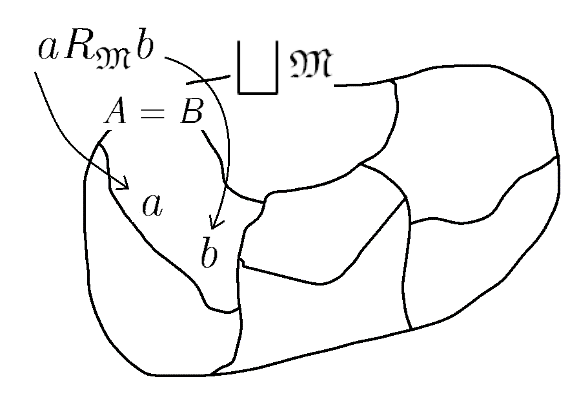
\includegraphics[width=160pt]{1.2.5.a.png}
\end{center}
\begin{dfn}
集合$A$の1つの同値関係$R$が与えられたとする。このとき、次式のような集合$C_{R}(a)$が定義されよう。
\begin{align*}
C_{R}(a) = \left\{ c \in A \middle| aRc \right\} \subseteq A
\end{align*}
この集合$C_{R}(a)$をその同値関係$R$によるその元$a$の同値類、または単に、類などといい$[ a]_{R}$、$\overline{a}$などとも書く。
\end{dfn}\par
このことは次のようにして考えられればわかりやすかろう。
\begin{center}
  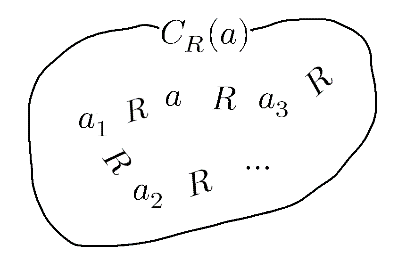
\includegraphics[width=160pt]{1.2.5.b.png}
\end{center}
\begin{thm}\label{8.1.4.29}
次のことが成り立つ。
\begin{itemize}
\item
  $\forall a \in A$に対し、$a \in C_{R}(a)$が成り立つ。
\item
  $\forall a,b \in A$に対し、$aRb$が成り立つならそのときに限り、$C_{R}(a) = C_{R}(b)$が成り立つ。
\item
  $\forall a,b \in A$に対し、$C_{R}(a) \neq C_{R}(b)$が成り立つなら、$C_{R}(a) \cap C_{R}(b) = \emptyset$が成り立つ。
\end{itemize}
\end{thm}
\begin{thm}\label{8.1.4.30}
集合$A$の1つの同値関係$R$が与えられたとする。次式のようにその同値関係$R$によるその元$a$の同値類全体の集合$\mathfrak{M}$が定義されると、
\begin{align*}
\mathfrak{M}=\left\{ C_{R}(a)\in \mathfrak{P}(A) \middle| C_{R}(a) = \left\{ c \in A \middle| aRc \right\} \right\}
\end{align*}
その集合$\mathfrak{M}$はその集合$A$の直和分割でこれに付随する同値関係$R_{\mathfrak{M}}$はその同値関係$R$に等しい。
\end{thm}\par
このことは次のようにして考えられればわかりやすかろう。
\begin{center}
    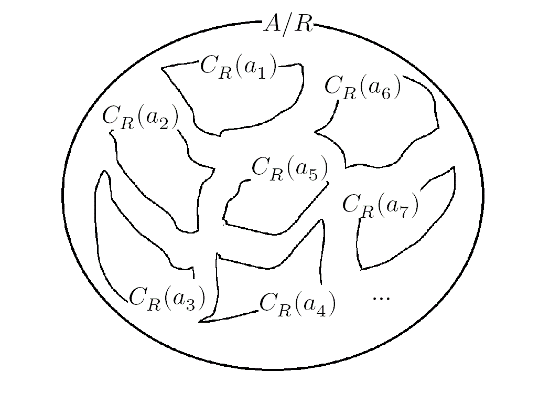
\includegraphics[width=160pt]{1.2.5.c.png}
\end{center}
\begin{dfn}
このようにして、その同値関係$R$からその集合$\mathfrak{M}$が定義されること、即ち、その集合$A$がその同値関係$R$によって得られる同値類たちの直和$\bigsqcup_{} \mathfrak{M}$とみなすことをその集合$A$のその同値関係$R$による類別、分類といいその集合$\mathfrak{M}$をその集合$A$のその同値関係による商集合といい$A/R$などと書く。
\end{dfn}
\begin{thm}\label{8.1.4.31}
ここで、写像$f:A \rightarrow B$が与えられたとする。このとき、その集合$A$の元々$a$、$b$に対し、次式のように論理式$aR(f)b$が定義されると、
\begin{align*}
aR(f)b \Leftrightarrow a,b \in A \land f(a) = f(b)
\end{align*}
その集合$A$における関係$R(f)$が得られこれは同値関係となる。
\end{thm}
\begin{dfn}
この関係$R(f)$をその写像$f$に付随する同値関係、その写像$f$の同値核などという。
\end{dfn}
\begin{thm}\label{8.1.4.32}
集合$A$の1つの同値関係$R$が与えられたとする。次式のように写像$C_{R}$が定義されるとき、
\begin{align*}
C_{R}:A \rightarrow A/R;a \mapsto C_{R}(a)
\end{align*}
その写像$C_{R}$は全射でありこれに付随する同値関係$R\left( C_{R} \right)$はその同値関係$R$に等しい。
\end{thm}
\begin{dfn}
このような写像$C_{R}$をその集合$A$からその集合$A/R$への標準的全射、自然な全射、商写像などという。
\end{dfn}
\end{comment}
\begin{dfn}
位相空間$\left( S,\mathfrak{O} \right)$と同値関係$R$が与えられたとき、その標準的全射$C_{R}:S \rightarrow {S}/{R};a \mapsto C_{R}(a)$を用いて次式のように集合$\overline{\mathfrak{O}}$が定義される。この集合$\overline{\mathfrak{O}}$を位相空間$\left( S.\mathfrak{O} \right)$の同値関係$R$における商位相という。
\begin{align*}
\overline{\mathfrak{O}} = \left\{ O \in \mathfrak{P}\left( {S}/{R} \right) \middle| V\left( C_{R}^{- 1}|O \right)\in \mathfrak{O} \right\}
\end{align*}
\end{dfn}
\begin{thm}\label{8.1.4.33}
組$\left( {S}/{R},\overline{\mathfrak{O}} \right)$は位相空間である。
\end{thm}
\begin{dfn}
この位相空間$\left( {S}/{R},\overline{\mathfrak{O}} \right)$を位相空間$\left( S.\mathfrak{O} \right)$の同値関係$R$における商位相空間という。
\end{dfn}
\begin{proof}
上記のように定義された組$\left( {S}/{R},\overline{\mathfrak{O}} \right)$において、次のようになることから、
\begin{align*}
V\left( C_{R}^{- 1}|{S}/{R} \right) = V\left( C_{R}^{- 1} \right) = D\left( C_{R} \right) = S,\ \ V\left( C_{R}^{- 1}|\emptyset \right) = \emptyset
\end{align*}
${S}/{R},\emptyset \in \overline{\mathfrak{O}}$が成り立つ。$\forall O,P \in \overline{\mathfrak{O}}$に対し、$V\left( C_{R}^{- 1}|O \right),V\left( C_{R}^{- 1}|P \right)\in \mathfrak{O}$が成り立つので、次のようになる。
\begin{align*}
V\left( C_{R}^{- 1}|O \right) \cap V\left( C_{R}^{- 1}|P \right) = V\left( C_{R}^{- 1}|O \cap P \right)\in \mathfrak{O}
\end{align*}
したがって、$O \cap P \in \overline{\mathfrak{O}}$が成り立つ。任意の添数集合$\varLambda$によって添数づけられたその商位相$\overline{\mathfrak{O}}$の族$\left\{ O_{\lambda} \right\}_{\scriptsize \begin{matrix}
\lambda \in \varLambda \\
\end{matrix}}$が与えられたとき、$\forall\lambda \in \varLambda$に対し、$V\left( C_{R}^{- 1}|O_{\lambda} \right)\in \mathfrak{O}$が成り立つので、次のようになる。
\begin{align*}
\bigcup_{\scriptsize \begin{matrix}
\lambda \in \varLambda \\
\end{matrix}} {V\left( C_{R}^{- 1}|O_{\lambda} \right)} = V\left( C_{R}^{- 1}|\bigcup_{\scriptsize \begin{matrix}
\lambda \in \varLambda \\
\end{matrix}} O_{\lambda} \right)\in \mathfrak{O}
\end{align*}
したがって、$\bigcup_{\scriptsize \begin{matrix}
\lambda \in \varLambda \\
\end{matrix}} O_{\lambda} \in \overline{\mathfrak{O}}$が成り立つ。以上より、その組$\left( {S}/{R},\overline{\mathfrak{O}} \right)$は位相空間である。
\end{proof}
\begin{thm}\label{8.1.4.34}
位相空間$\left( S.\mathfrak{O} \right)$の同値関係$R$における商位相空間$\left( {S}/{R},\overline{\mathfrak{O}} \right)$が与えられたとき、標準的全射$C_{R}:S \rightarrow {S}/{R};a \mapsto C_{R}(a)$はその位相空間$\left( S,\mathfrak{O} \right)$からその商位相空間$\left( {S}/{R},\overline{\mathfrak{O}} \right)$への連続写像である。
\end{thm}
\begin{proof}
位相空間$\left( S.\mathfrak{O} \right)$の同値関係$R$における商位相空間$\left( {S}/{R},\overline{\mathfrak{O}} \right)$が与えられたとき、その標準的全射$C_{R}:S \rightarrow {S}/{R};a \mapsto C_{R}(a)$について、商位相の定義より明らかに、$\forall O \in \overline{\mathfrak{O}}$に対し、$V\left( C_{R}^{- 1}|O \right)\in \mathfrak{O}$が成り立つので、その標準的全射$C_{R}:S \rightarrow {S}/{R};a \mapsto C_{R}(a)$はその位相空間$\left( S,\mathfrak{O} \right)$からその商位相空間$\left( {S}/{R},\overline{\mathfrak{O}} \right)$への連続写像である。
\end{proof}
\begin{thm}\label{8.1.4.35}
位相空間たち$\left( S,\mathfrak{O} \right)$、$\left( T,\mathfrak{P} \right)$とそれらの間の連続写像$f:S \rightarrow T$、その集合$S$におけるその写像$f$に付随する同値関係$R(f)$が与えられたとき、次式のような写像$\overline{f}$が定まりこれはその商位相空間$\left( {S}/{R(f)},\overline{\mathfrak{O}} \right)$からその位相空間$\left( T,\mathfrak{P} \right)$への連続写像となる。
\begin{align*}
\overline{f}:{S}/{R(f)} \rightarrow T;C_{R(f)}(a) \mapsto f(a)
\end{align*}
\end{thm}
\begin{proof}
位相空間たち$\left( S,\mathfrak{O} \right)$、$\left( T,\mathfrak{P} \right)$とそれらの間の連続写像$f:S \rightarrow T$、その集合$S$におけるその写像$f$に付随する同値関係$R(f)$が与えられたとき、次式のような対応$\overline{f}$について考えよう。
\begin{align*}
\overline{f} = \left( {S}/{R(f)},T,G \right),\ \ G = \left\{ \left( C_{R(f)}(a),b \right) \in {S}/{R(f)} \times T \middle| b = f(a) \right\}
\end{align*}
このとき、$\forall C_{R(f)}(a),C_{R(f)}(b) \in {S}/{R(f)}$に対し、$C_{R(f)}(a) = C_{R(f)}(b)$が成り立つなら、$aR(f)b$が成り立ち、したがって、$f(a) = f(b)$も成り立つ。したがって、その対応$\overline{f}$は写像である。このとき、標準的全射$C_{R(f)}:S \rightarrow {S}/{R(f)};a \mapsto C_{R(f)}(a)$を用いて$f = \overline{f} \circ C_{R(f)}$が成り立つことに注意すれば、$\forall P \in \mathfrak{P}$に対し、$V\left( f^{- 1}|P \right)\in \mathfrak{O}$が成り立ち、ここで、$f^{- 1} = C_{R(f)}^{- 1} \circ {\overline{f}}^{- 1}$が成り立つので、$V\left( C_{R(f)}^{- 1}|V\left( {\overline{f}}^{- 1}|P \right) \right)\in \mathfrak{O}$が成り立つ。したがって、定義より明らかにその同値関係$R$による商位相$\overline{\mathfrak{O}}$を用いて$V\left( {\overline{f}}^{- 1}|P \right) \in \overline{\mathfrak{O}}$が得られるので、その写像$\overline{f}$はその商位相空間$\left( {S}/{R(f)},\overline{\mathfrak{O}} \right)$からその位相空間$\left( T,\mathfrak{P} \right)$への連続写像となる。
\end{proof}
\begin{thm}\label{8.1.4.36}
位相空間たち$\left( S,\mathfrak{O} \right)$、$\left( T,\mathfrak{P} \right)$とそれらの間の連続写像$f:S \rightarrow T$、それらの集合たち$S$、$T$における同値関係たち$Q$、$R$が与えられ、$\forall a,b \in S$に対し、$aQb$が成り立つなら、$f(a)Rf(b)$が成り立つとき、次式のような写像$\overline{f}$が定まりこれはその商位相空間$\left( {S}/{Q},\overline{\mathfrak{O}} \right)$からその商位相空間$\left( {T}/{R},\overline{\mathfrak{P}} \right)$への連続写像となる。
\begin{align*}
\overline{f}:{S}/{Q} \rightarrow {T}/{R};C_{Q}(a) \mapsto C_{R} \circ f(a)
\end{align*}
\end{thm}
\begin{proof}
位相空間たち$\left( S,\mathfrak{O} \right)$、$\left( T,\mathfrak{P} \right)$とそれらの間の連続写像$f:S \rightarrow T$、それらの集合たち$S$、$T$における同値関係たち$Q$、$R$が与えられ、$\forall a,b \in S$に対し、$aQb$が成り立つなら、$f(a)Rf(b)$が成り立つとき、次式のような対応$\overline{f}$について考えよう。
\begin{align*}
\overline{f} = \left( {S}/{Q},{T}/{R},G \right),\ \ G = \left\{ \left( C_{Q}(a),C \right) \in {S}/{Q} \times {T}/{R} \middle| C = C_{R} \circ f(a) \right\}
\end{align*}
このとき、$\forall C_{Q}(a),C_{Q}(b) \in {S}/{Q}$に対し、$C_{Q}(a) = C_{Q}(b)$が成り立つなら、$aQb$が成り立ち、したがって、$f(a)Rf(b)$も成り立つので、$C_{R} \circ f(a) = C_{R} \circ f(b)$も成り立つ。したがって、その対応$\overline{f}$は写像である。ここで、定理\ref{8.1.4.34}よりその商位相空間$\left( {T}/{R},\overline{\mathfrak{P}} \right)$を用いた標準的全射$C_{R}:T \rightarrow {T}/{R};a \mapsto C_{R}(a)$はその位相空間$\left( T,\mathfrak{P} \right)$からその商位相空間$\left( {T}/{R},\overline{\mathfrak{P}} \right)$への連続写像となるのであった。このとき、その合成写像$C_{R} \circ f:S \rightarrow {T}/{R}$も連続写像で定理\ref{8.1.4.35}よりその写像$\overline{f}:{S}/{Q} \rightarrow {T}/{R};C_{Q}(a) \mapsto C_{R} \circ f(a)$も連続写像となる。
\end{proof}
\begin{thebibliography}{50}
\bibitem{1}
  松坂和夫, 集合・位相入門, 岩波書店, 1968. 新装版第2刷 p52-59,186-194 ISBN978-4-00-029871-1
\bibitem{2}
  加塩朋和. "一般位相A(2組)". 東京理科大学. \url{https://www.rs.tus.ac.jp/a25594/2018-2019_General_Topology.pdf} (2021-8-6 12:15 取得)
\end{thebibliography}
\end{document}
